\setcounter{definition}{0} \setcounter{property}{0} \setcounter{claim}{0} \setcounter{fact}{0} \setcounter{corollary}{0} \setcounter{figure}{0}
\section{NP-complete}

\begin{definition}[NP-complete]
Let $X$ be a decision problem. We say $X$ is NP-complete, if $X$ is in NP, and for every problem $X'$ in NP, we have $X'\le_p X$.
\end{definition}

NP-complete problems are the ``hardest'' problems in NP. It's not obvious that
NP-complete problems even exist.
Thanks to the pioneers of computer science: in 1971 Cook and Levin proved the first
NP-complete problem by showing that the \emph{satisfiability problem} is NP-complete.
This builds the foundation of complexity theory.

The satisfiability~(SAT) problem is
to decide if a given boolean formula can be satisfied
by assigning values to boolean variables.
Let's define it. The \emph{variables}, $x_1, x_2, \cdots, x_m$, involved are
boolean~(or binary), taking value of either true or false.
A \emph{literal} is either a variable itself~(e.g., $x_3$, $x_5$, etc) or the negation of a variable~(e.g., $\overline{x_3}$, $\overline{x_5}$, etc).
A \emph{clause} is a disjunction of literals~(e.g., $x_2 \vee \overline{x_4}$, $\overline{x_3} \vee \overline{x_5} \vee x_2$, $\overline{x_1}$, etc).
A \emph{CNF~(conjunctive normal form) formula} is a conjunction of clauses, such as
$(x_2 \vee \overline{x_4})\wedge (\overline{x_3} \vee \overline{x_5} \vee x_2) \wedge (\overline{x_1})$.

Given a CNF formula with $n$ clauses $C_1, C_2, \cdots, C_n$ involving $m$ variables
$x_1, x_2, \cdots, x_m$, the SAT problem is to decide if there exists an
\emph{assignment}~(i.e., assigning true or false value to each variable) such
that all $n$ clauses are true~(i.e., the CNF formula is true).

If each clause is restricted to have exactly 3 literals, then the above problem becomes the so-called 3SAT problem.
3SAT has been proved to be NP-hard, i.e., there doesn't exist any efficient algorithm for it unless P~=~NP.
(We will introduce NP-completeness later this course; you don't need to know that these mean now.)

If each clause is restricted to have exactly 2 literals, then the above problem becomes the 2SAT problem.
2SAT can be solved in polynomial-time.
If each clause is restricted to have exactly 3 literals, then the above problem becomes the so-called 3SAT problem.
3SAT has been proved to be NP-hard.
Below, we only prove its first part, i.e., 3SAT is in NP.
%Below we will design an algorithm for 2SAT, in which the core part is to use the algorithm of identifying connected componenets of directed graphs.


\begin{fact}
3SAT problem is in NP.
\end{fact}
\emph{Proof.} By definition, to prove 3SAT is in NP, we need to design an
algorithm~(i.e., the verifier $A$), and show that it satisfies the two
conditions. For 3SAT, the certificate is an assignment for all variables,
which can be represented as a binary vector. The verifier, given below, will check
if the given binary vector is in correct length, and if it satisfies all clauses,
and these can be done in polynomial-time.

\begin{minipage}{0.8\textwidth}
	\aaA {4}{verifier~$(x, c)$}\xxx
	\aab {verify that the length of $c$ equals to the number of variables in instance $x$: if not, return ``no'';}\xxx
	\aab {verify that every clause in instance $x$ is true when $x_i$ is assigned with $c[i]$: if not, return ``no'';}\xxx
	\aab {return ``yes'';}\xxx
	\aaa {end;}\xxx
\end{minipage}

Now we prove that above verifier satisfies the two conditions.
It clearly takes an instance and a certificate as input.
If $x$ is an ``true''-instance, then it means $x$ is satisfiable, i.e.,
there exists an assignment that satisfies all clauses.
Clearly, once this assignment is passed to the verifier together with $x$,
the verifier will return ``yes''.
If $x$ is an ``false''-instance, then it means $x$ is not satisfiable, i.e.,
there does not exist an assignment that satisfies all clauses.
Hence, no matter what is passed to the verifier with $x$,
the verifier always returns ``no''. Also, verifier $A$ runs in polynomial-time.
This proves that 3SAT is in NP.
\qed




We study how to prove that a problem is NP-complete by reducing from known
NP-complete problems. The approach is based on the following key idea.

\begin{fact}
Let $Y$ be a problem in NP. If there exists an NP-complete problem $X$ such that $X\le_p Y$,
then $Y$ is NP-complete.
\end{fact}

This is intuitive: $X$ is NP-complete, i.e., it is (one of) the hardest problem
in NP; of course $X$ is at least as hard as $Y$ because $Y$ is in NP.
Now we have $X\le_p Y$, i.e., $Y$ is at least as hard as $X$. Combined, $Y$ is (one of) the
hardest problem in NP as well. Below we give a formal proof.

\emph{Proof.} Let $X'$ an arbitrary problem in NP. Since problem $X$ is NP-complete,
by definition, we have $X' \le_p X$. Since $X\le_p Y$, we must have that $X'\le Y$.
(Here we use the property that the polynomial-time reduction is transitive, i.e.,
 if $A\le_p B$ and $B\le_p C$ then $A\le_p C$.)
Combining that $Y$ is in NP, we know that $Y$ is NP-complete.\qed

Above Fact suggest a procedure to prove that a decision problem $Y$ is NP-complete.
\begin{enumerate}
\item Show that $Y$ is in NP;
\item Pick an existing NP-complete problem $X$;
\item Show that $X$ is polynomial-time reducible to $Y$. 
\end{enumerate}

Below we give two examples. So far, we (only) know one NP-complete
problem, 3SAT. We will use it for proving other problems to be NP-complete.

%Using above procedure, lots of problems have been proved to be NP-complete.
%These includes the 3SAT problem, the decision-version of the vertex cover problem, i.e., $VC(G,k)$.
%Other well-known NP-complete problems include, the decision-version of independenet set problem,
%the Hamiltonian path problem, 
%the Hamiltonian cycle problem, 
%3D matching problem, $k$-coloring problem when $k\ge 3$, the subset-sum problem, decision-version of TSP~(traveling salesman problems), etc.
%Below we give some details for the independent set problem.

\subsection*{Independent Set}

An \emph{independent set} of an undirected graph $G = (V, E)$
is a subset of vertices $V_1\subset V$ satisfying that no two vertices in it is connected by an edge, i.e.,
for any $u,v\in V_1$, we have $(u,v)\not\in E$. We define two versions of the independent set problem.
\begin{enumerate}
\item optimization-version: given an undirected graph $G = (V, E)$, to seek an independent set $V_1$ of $G$ such that $V_1$ is maximized; we denote this problem as $IS(G)$;
\item decision-version: given an undirected graph $G = (V, E)$ and integer $k\ge 0$, to decide if there exists an independent set $V_1$ of $G$ such that $|V_1| \ge k$;
we denote this problem as $IS(G,k)$.
\end{enumerate}

There is a simple connection between independent set and vertex cover. 
See Figure~\ref{fig:is} for an example.
(Can you spot it?) 

\begin{fact}
Let $G = (V, E)$ be an undirected graph. We have $V_1\subset V$ is an independent set of $G$ if and only if $V\setminus V_1$ is a vertex cover of $G$.
\end{fact}

\begin{figure}[!h]
\centering{\input{is}}
\caption{Relationship between independent set and vertex cover.}
\label{fig:is}
\end{figure}

Above fact immediately suggests the following corollaries.
\begin{corollary}
$V_1^*\subset V$ is one maximum independent set of an undirected graph $G$ if and only if $V\setminus V_1^*$ is one minimum vertex cover of $G$.
\end{corollary}
\begin{corollary}
$G$ has an independent set with $k$ vertices if and only if $G$ has a vertex cover with $|V|-k$ vertices.
\end{corollary}

According to Corollary~2, we have $VC(G, k) \le_p IS(G, k)$, as we can design
an algorithm for $VC(G,k)$ with one statement ``return
solver-for-$IS(G,|V|-k)$''.
%Note that, this actually proves that $IS(G,k)$ is NP-complete, given that $VC(G,k)$ is NP-complete and $IS(G,k)$ is in NP.
Symmetrically we have $IS(G,k)\le_p VC(G,k)$.
Similarly, according to Corollary~1, we can write $IS(G) \le_p VC(G)$ and $VC(G) \le_p IS(G)$.
Recall that we also proved that $VC(G,k)\le_p VC(G)$ and $VC(G)\le_p VC(G,k)$. % in Lecture~41.
We conclude that all the four problems are equivalent, i.e., any two of them are polynomial-time reducible to each other.

We now prove that, $IS(G, k)$ is NP-complete.
The first step is to show that this problem is in NP.
The certificate is a solution, in this case an independent set $V_1$ of $G$ of size at least $k$.
The verifier takes $G$, $k$, and certificate $c$ as input, and verifies (1), whether $c$ is a subset of vertices of $G$,
(2), whether $c$ is an indepdent set, i.e., no two vertices in it are connected by an edge,
and (3), whether the size of $c$ is at least $k$. If all these are satisfied, the verifier returns ``yes'' and otherwise ''no''.
Clearly, if the instance ($G,k$) is a ``true'' instance, meaning that there exists an independent set $V_1$ of size at least $k$,
then verifier will return ``yes'' when given $G$, $k$ together with $V_1$ as input.
On the other side, if the instance ($G,k$) is a ``false'' instance, which means that there 
does not exist an independent set $V_1$ of size at least $k$, then the verifier will always output ``no''.

Next, we pick an existing NP-complete problem $X$ and show that $X$ is polynomial-time reducible to $IS(G, k)$.
The choice for $X$ here is 3SAT.
We therefore need to design an algorithm for 3SAT, assuming and using (up to polynomial-time) an algorithm for $IS(G, k)$.
Here is a way of interpreting both problems that bridges them.
\begin{enumerate}
\vspace*{-\topsep}
\item An instance of 3SAT is satisfiable~(i.e., a ``true'' instance), if and only if, one can pick a literal in each clause such that 
a variable and its negation are not picked simultaneously. To see this formally, if a 3SAT instance is satisfiable,
there exists an assignment for all variables such that at least one literal in each clause is true. We can then pick
a true literal from each clause. The picked literals certainly cannot include both $x$ and $\overline{x}$ as they cannot
be true at the same time. On the other side, assume that one can pick a literal in each clause such that 
no variable and its negation are both chosen.  Letting all these $n$ literals be true satisfy all clauses. 
For each variable $x$,
if literal $x$ gets picked, we assign $x$ to be true; if $\overline{x}$ is picked we assign $x$ to be false; if
none of these two we assign $x$ a random value. Clearly, this assignment to all variables satisfy all clauses. 
\item An instance of $IS(G,k)$ is a ``true'' instane, if and only if, one can pick $k$ vertices in $G$ such that
the two ends of an edge are not picked simultaneously.
\end{enumerate}

Above analysis suggests that, for a 3SAT instance we build a graph $G$ with
vertices representing literals and edges connecting variables and their negations.
Formally, assume the given 3SAT instance consists of $m$ variables $x_1, x_2, \cdots, x_m$
and $n$ clauses $C_1, C_2, \cdots, C_n$. We build an undirected graph $G$ with $3n$ vertices which
correspond to the $3n$ literals in the $n$ clauses. We add an edge for any two literals/vertices
in the form of a variable $x$ and its negation $\overline{x}$.
Finally, we add 3 edges to connect the 3 pairs of literals in each clause.
See Figure~\ref{fig:3satis}. The algorithm (for 3SAT) calls a solver for $IS(G,k)$
to decide if the constructed graph $G$ has an independent set of size at least $n$.
If ``yes'' the algorithm return ``yes'', and returns ``no'' otherwise.

\begin{figure}[!h]
\centering{

\tikzset{every picture/.style={line width=0.75pt}} %set default line width to 0.75pt        

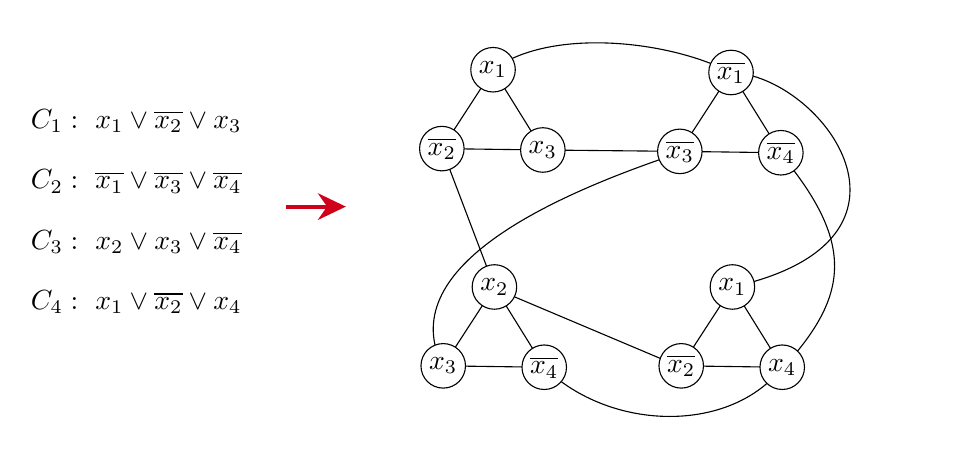
\begin{tikzpicture}[x=0.5pt,y=0.5pt,yscale=-1,xscale=1]
%uncomment if require: \path (0,313); %set diagram left start at 0, and has height of 313

%Straight Lines [id:da6618167296725836] 
\draw    (416.92,104.08) -- (515.92,105.08) ;
%Curve Lines [id:da22396963516709756] 
\draw    (589.92,261.08) .. controls (553,309) and (466,308) .. (417.92,261.08) ;
%Straight Lines [id:da4039573391796768] 
\draw    (343.92,103.08) -- (381.92,203.08) ;
%Straight Lines [id:da13937003486319577] 
\draw    (381.92,204.08) -- (516.92,261.08) ;
%Curve Lines [id:da866328606831125] 
\draw    (344.92,261.08) .. controls (308,190) and (420,138) .. (515.92,106.08) ;
%Curve Lines [id:da9209425626994789] 
\draw    (588.92,107.08) .. controls (642,171) and (639,209) .. (589.92,262.08) ;
%Curve Lines [id:da4940637759678749] 
\draw    (552.92,48.08) .. controls (618,50) and (708,169) .. (553.92,203.08) ;
%Curve Lines [id:da5522864666968264] 
\draw    (380.92,46.08) .. controls (420.92,16.08) and (506,24) .. (552.92,48.08) ;
%Straight Lines [id:da39949851653001356] 
\draw    (343.92,103.08) -- (416.92,104.08) ;
%Straight Lines [id:da06151606308920077] 
\draw    (380.92,46.08) -- (416.92,104.08) ;
%Straight Lines [id:da6053357926244952] 
\draw    (343.92,103.08) -- (380.92,46.08) ;
%Shape: Ellipse [id:dp6988649017460684] 
\draw  [fill={rgb, 255:red, 255; green, 255; blue, 255 }  ,fill opacity=1 ] (327.83,103.08) .. controls (327.83,94.19) and (335.03,86.99) .. (343.92,86.99) .. controls (352.8,86.99) and (360,94.19) .. (360,103.08) .. controls (360,111.96) and (352.8,119.16) .. (343.92,119.16) .. controls (335.03,119.16) and (327.83,111.96) .. (327.83,103.08) -- cycle ;
%Shape: Ellipse [id:dp6915506911604865] 
\draw  [fill={rgb, 255:red, 255; green, 255; blue, 255 }  ,fill opacity=1 ] (400.83,104.08) .. controls (400.83,95.19) and (408.03,87.99) .. (416.92,87.99) .. controls (425.8,87.99) and (433,95.19) .. (433,104.08) .. controls (433,112.96) and (425.8,120.16) .. (416.92,120.16) .. controls (408.03,120.16) and (400.83,112.96) .. (400.83,104.08) -- cycle ;
%Shape: Ellipse [id:dp4366461272272538] 
\draw  [fill={rgb, 255:red, 255; green, 255; blue, 255 }  ,fill opacity=1 ] (364.83,46.08) .. controls (364.83,37.19) and (372.03,29.99) .. (380.92,29.99) .. controls (389.8,29.99) and (397,37.19) .. (397,46.08) .. controls (397,54.96) and (389.8,62.16) .. (380.92,62.16) .. controls (372.03,62.16) and (364.83,54.96) .. (364.83,46.08) -- cycle ;
%Straight Lines [id:da042710010547382216] 
\draw    (515.92,105.08) -- (588.92,106.08) ;
%Straight Lines [id:da8892833055324549] 
\draw    (552.92,48.08) -- (588.92,106.08) ;
%Straight Lines [id:da0818748968414269] 
\draw    (515.92,105.08) -- (552.92,48.08) ;
%Shape: Ellipse [id:dp3629673290953376] 
\draw  [fill={rgb, 255:red, 255; green, 255; blue, 255 }  ,fill opacity=1 ] (499.83,105.08) .. controls (499.83,96.19) and (507.03,88.99) .. (515.92,88.99) .. controls (524.8,88.99) and (532,96.19) .. (532,105.08) .. controls (532,113.96) and (524.8,121.16) .. (515.92,121.16) .. controls (507.03,121.16) and (499.83,113.96) .. (499.83,105.08) -- cycle ;
%Shape: Ellipse [id:dp13012257517742154] 
\draw  [fill={rgb, 255:red, 255; green, 255; blue, 255 }  ,fill opacity=1 ] (572.83,106.08) .. controls (572.83,97.19) and (580.03,89.99) .. (588.92,89.99) .. controls (597.8,89.99) and (605,97.19) .. (605,106.08) .. controls (605,114.96) and (597.8,122.16) .. (588.92,122.16) .. controls (580.03,122.16) and (572.83,114.96) .. (572.83,106.08) -- cycle ;
%Shape: Ellipse [id:dp4087408185133151] 
\draw  [fill={rgb, 255:red, 255; green, 255; blue, 255 }  ,fill opacity=1 ] (536.83,48.08) .. controls (536.83,39.19) and (544.03,31.99) .. (552.92,31.99) .. controls (561.8,31.99) and (569,39.19) .. (569,48.08) .. controls (569,56.96) and (561.8,64.16) .. (552.92,64.16) .. controls (544.03,64.16) and (536.83,56.96) .. (536.83,48.08) -- cycle ;
%Straight Lines [id:da3279698789670312] 
\draw    (344.92,260.08) -- (417.92,261.08) ;
%Straight Lines [id:da13651038513236746] 
\draw    (381.92,203.08) -- (417.92,261.08) ;
%Straight Lines [id:da07037214338199449] 
\draw    (344.92,260.08) -- (381.92,203.08) ;
%Shape: Ellipse [id:dp040453670796765206] 
\draw  [fill={rgb, 255:red, 255; green, 255; blue, 255 }  ,fill opacity=1 ] (328.83,260.08) .. controls (328.83,251.19) and (336.03,243.99) .. (344.92,243.99) .. controls (353.8,243.99) and (361,251.19) .. (361,260.08) .. controls (361,268.96) and (353.8,276.16) .. (344.92,276.16) .. controls (336.03,276.16) and (328.83,268.96) .. (328.83,260.08) -- cycle ;
%Shape: Ellipse [id:dp4286753979995753] 
\draw  [fill={rgb, 255:red, 255; green, 255; blue, 255 }  ,fill opacity=1 ] (401.83,261.08) .. controls (401.83,252.19) and (409.03,244.99) .. (417.92,244.99) .. controls (426.8,244.99) and (434,252.19) .. (434,261.08) .. controls (434,269.96) and (426.8,277.16) .. (417.92,277.16) .. controls (409.03,277.16) and (401.83,269.96) .. (401.83,261.08) -- cycle ;
%Shape: Ellipse [id:dp772850742920124] 
\draw  [fill={rgb, 255:red, 255; green, 255; blue, 255 }  ,fill opacity=1 ] (365.83,203.08) .. controls (365.83,194.19) and (373.03,186.99) .. (381.92,186.99) .. controls (390.8,186.99) and (398,194.19) .. (398,203.08) .. controls (398,211.96) and (390.8,219.16) .. (381.92,219.16) .. controls (373.03,219.16) and (365.83,211.96) .. (365.83,203.08) -- cycle ;
%Straight Lines [id:da5751805739442735] 
\draw    (516.92,260.08) -- (589.92,261.08) ;
%Straight Lines [id:da5903012678345287] 
\draw    (553.92,203.08) -- (589.92,261.08) ;
%Straight Lines [id:da38407080032275986] 
\draw    (516.92,260.08) -- (553.92,203.08) ;
%Shape: Ellipse [id:dp5500860302509325] 
\draw  [fill={rgb, 255:red, 255; green, 255; blue, 255 }  ,fill opacity=1 ] (500.83,260.08) .. controls (500.83,251.19) and (508.03,243.99) .. (516.92,243.99) .. controls (525.8,243.99) and (533,251.19) .. (533,260.08) .. controls (533,268.96) and (525.8,276.16) .. (516.92,276.16) .. controls (508.03,276.16) and (500.83,268.96) .. (500.83,260.08) -- cycle ;
%Shape: Ellipse [id:dp9081445012691336] 
\draw  [fill={rgb, 255:red, 255; green, 255; blue, 255 }  ,fill opacity=1 ] (573.83,261.08) .. controls (573.83,252.19) and (581.03,244.99) .. (589.92,244.99) .. controls (598.8,244.99) and (606,252.19) .. (606,261.08) .. controls (606,269.96) and (598.8,277.16) .. (589.92,277.16) .. controls (581.03,277.16) and (573.83,269.96) .. (573.83,261.08) -- cycle ;
%Shape: Ellipse [id:dp7856009471528769] 
\draw  [fill={rgb, 255:red, 255; green, 255; blue, 255 }  ,fill opacity=1 ] (537.83,203.08) .. controls (537.83,194.19) and (545.03,186.99) .. (553.92,186.99) .. controls (562.8,186.99) and (570,194.19) .. (570,203.08) .. controls (570,211.96) and (562.8,219.16) .. (553.92,219.16) .. controls (545.03,219.16) and (537.83,211.96) .. (537.83,203.08) -- cycle ;
%Straight Lines [id:da14088417165595923] 
\draw [color={rgb, 255:red, 208; green, 2; blue, 27 }  ,draw opacity=1 ][line width=1.5]    (231.5,145) -- (270.5,145) ;
\draw [shift={(274.5,145)}, rotate = 180] [fill={rgb, 255:red, 208; green, 2; blue, 27 }  ,fill opacity=1 ][line width=0.08]  [draw opacity=0] (20.36,-9.78) -- (0,0) -- (20.36,9.78) -- (13.52,0) -- cycle    ;

% Text Node
\draw (45,73) node [anchor=north west][inner sep=0.75pt]   [align=left] {$\displaystyle C_{1} :\ x_{1} \lor \overline{x_{2}} \lor x_{3}$};
% Text Node
\draw (45,116.67) node [anchor=north west][inner sep=0.75pt]   [align=left] {$\displaystyle C_{2} :\ \overline{x_{1}} \lor \overline{x_{3}} \lor \overline{x_{4}}$};
% Text Node
\draw (45,160.34) node [anchor=north west][inner sep=0.75pt]   [align=left] {$\displaystyle C_{3} :\ x_{2} \lor x_{3} \lor \overline{x_{4}}$};
% Text Node
\draw (45,204) node [anchor=north west][inner sep=0.75pt]   [align=left] {$\displaystyle C_{4} :\ x_{1} \lor \overline{x_{2}} \lor x_{4}$};
% Text Node
\draw (380.92,46.08) node   [align=left] {$\displaystyle x_{1}$};
% Text Node
\draw (552.92,48.08) node   [align=left] {$\displaystyle \overline{x_{1}}$};
% Text Node
\draw (381.92,203.08) node   [align=left] {$\displaystyle x_{2}$};
% Text Node
\draw (343.92,103.08) node   [align=left] {$\displaystyle \overline{x_{2}}$};
% Text Node
\draw (416.92,104.08) node   [align=left] {$\displaystyle x_{3}$};
% Text Node
\draw (515.92,105.08) node   [align=left] {$\displaystyle \overline{x_{3}}$};
% Text Node
\draw (588.92,106.08) node   [align=left] {$\displaystyle \overline{x_{4}}$};
% Text Node
\draw (417.92,261.08) node   [align=left] {$\displaystyle \overline{x_{4}}$};
% Text Node
\draw (344.92,260.08) node   [align=left] {$\displaystyle x_{3}$};
% Text Node
\draw (553.92,203.08) node   [align=left] {$\displaystyle x_{1}$};
% Text Node
\draw (516.92,260.08) node   [align=left] {$\displaystyle \overline{x_{2}}$};
% Text Node
\draw (589.92,261.08) node   [align=left] {$\displaystyle x_{4}$};


\end{tikzpicture}

}
\caption{Reducing 3SAT to $IS(G,k)$. The 3SAT instance~(with $n$ clauses) is satisfiable
if and only if the resulting graph has an independent set of size $n$.}
\label{fig:3satis}
\end{figure}

To show the above algorithm is correct, we need to prove that the given 3SAT instance~(with $n$ clauses)
is satisfiable if and only if the constructed graph $G$ contains an independent set of size at least $n$.
%($\Longrightarrow$) 
Assume the 3SAT is satisfiable, i.e., one can pick $n$ literals, one from each clause, such that 
$x$ and $\overline{x}$ are not picked. In $G$, these $n$ literals/vertices
must form an independent set, since, according to how $G$ is constructed,
any two picked vertices will not be connected by the $(x,\overline{x})$ edge
nor by the edge connecting the literals within a clause~(because the picked literals
come from different clauses). To prove the other side, assume that $G$ contains
an independent set of size at least $n$. These vertices/literals must come from different clauses~(since
all literals within a clause are connected). 
So the size must be exactly $n$, one from each clause. 
Being independent guarantees that 
a variable and its negation, the two ends of an edge, must be not present simultaneously.



\subsection*{3D Matching}

3D matching generaizes the matching of bipartite graph~(i.e., 2D matching).
See Figure~\ref{fig:3dmatching}.
Formally, let $X$, $Y$, and $Z$ be 3 disjoint sets of vertices. 
A set $E\subset X\times Y \times Z$ is said to be \emph{edges},
each of which is a triple consists of 3 vertices from the 3 sets.
A matching $M$ of $(X,Y,Z,E)$ is a subset of $E$ such that
each vertex in $X\cup Y \cup Z$ appears in at most one edge in $E$;
in other words, any two edges in a matching does not share any vertex.

\begin{figure}[!h]
\centering{

\tikzset{every picture/.style={line width=0.75pt}} %set default line width to 0.75pt        

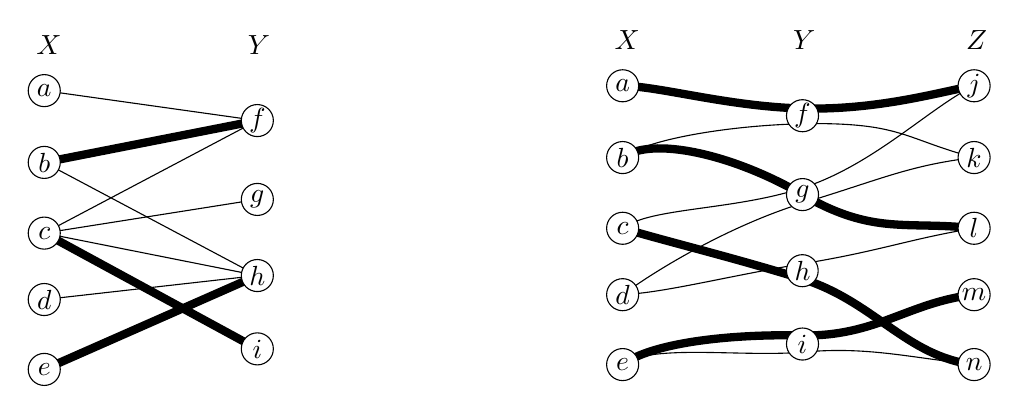
\begin{tikzpicture}[x=0.5pt,y=0.5pt,yscale=-1,xscale=1]
%uncomment if require: \path (0,292); %set diagram left start at 0, and has height of 292

%Curve Lines [id:da4241903757380898] 
\draw [line width=3]    (456.68,55.59) .. controls (484,56) and (534.03,70.9) .. (588,72) .. controls (641.97,73.1) and (686,60) .. (710.68,55.59) ;
%Curve Lines [id:da8255907428390687] 
\draw    (456.68,107.47) .. controls (477.18,92.09) and (551.03,81.9) .. (605,83) .. controls (658.97,84.1) and (664,95) .. (710.68,107.47) ;
%Curve Lines [id:da344500096054706] 
\draw    (456.68,158.57) .. controls (477.18,143.2) and (537,146) .. (588,129) .. controls (639,112) and (679,71) .. (710.68,55.59) ;
%Curve Lines [id:da11085604778848868] 
\draw    (456.68,206.57) .. controls (488,205) and (533,193) .. (588,184) .. controls (643,175) and (665,166) .. (710.68,158.57) ;
%Curve Lines [id:da7960793701320955] 
\draw [line width=3]    (456.68,257.08) .. controls (477.18,241.7) and (532.03,234.9) .. (586,236) .. controls (639.97,237.1) and (663,212) .. (710.68,206.57) ;
%Curve Lines [id:da9523105239538149] 
\draw    (456.68,257.08) .. controls (477.18,241.7) and (543,252) .. (588,248) .. controls (633,244) and (662,251.61) .. (710.68,257.08) ;
%Curve Lines [id:da7884208773008994] 
\draw [line width=3]    (456.68,107.47) .. controls (477.18,92.09) and (535.33,104.46) .. (586.67,134.23) .. controls (638,164) and (662,153.1) .. (710.68,158.57) ;
%Curve Lines [id:da943679960760185] 
\draw    (456.68,206.57) .. controls (477.18,191.2) and (532,157) .. (588,140) .. controls (644,123) and (664,113) .. (710.68,107.47) ;
%Curve Lines [id:da6807255577581136] 
\draw [line width=3]    (456.68,158.57) .. controls (488,168) and (534,179) .. (586,195) .. controls (638,211) and (662,251.61) .. (710.68,257.08) ;
%Straight Lines [id:da5756546325370752] 
\draw [line width=3]    (192.67,80.73) -- (38.68,110.97) ;
%Straight Lines [id:da9211662025642174] 
\draw    (38.68,59.09) -- (192.67,80.73) ;
%Straight Lines [id:da06434668113779485] 
\draw    (192.67,80.73) -- (38.68,162.07) ;
%Straight Lines [id:da4406012177704377] 
\draw    (192.67,192.73) -- (38.68,162.07) ;
%Straight Lines [id:da3723168518652895] 
\draw [line width=3]    (192.67,245.73) -- (38.68,162.07) ;
%Straight Lines [id:da746260912418035] 
\draw    (192.67,137.73) -- (38.68,162.07) ;
%Straight Lines [id:da9456704199726969] 
\draw    (192.67,192.73) -- (38.68,210.07) ;
%Straight Lines [id:da45949818054633906] 
\draw [line width=3]    (192.67,192.73) -- (38.68,260.58) ;
%Straight Lines [id:da9256706423252938] 
\draw    (192.67,192.73) -- (38.68,110.97) ;
%Shape: Ellipse [id:dp2702263199738577] 
\draw  [fill={rgb, 255:red, 255; green, 255; blue, 255 }  ,fill opacity=1 ] (27.1,260.58) .. controls (27.1,254.18) and (32.29,249) .. (38.68,249) .. controls (45.08,249) and (50.26,254.18) .. (50.26,260.58) .. controls (50.26,266.97) and (45.08,272.16) .. (38.68,272.16) .. controls (32.29,272.16) and (27.1,266.97) .. (27.1,260.58) -- cycle ;
%Shape: Ellipse [id:dp19077153467526664] 
\draw  [fill={rgb, 255:red, 255; green, 255; blue, 255 }  ,fill opacity=1 ] (27.1,110.97) .. controls (27.1,104.57) and (32.29,99.39) .. (38.68,99.39) .. controls (45.08,99.39) and (50.26,104.57) .. (50.26,110.97) .. controls (50.26,117.36) and (45.08,122.55) .. (38.68,122.55) .. controls (32.29,122.55) and (27.1,117.36) .. (27.1,110.97) -- cycle ;
%Shape: Ellipse [id:dp5053674258722656] 
\draw  [fill={rgb, 255:red, 255; green, 255; blue, 255 }  ,fill opacity=1 ] (27.1,162.07) .. controls (27.1,155.67) and (32.29,150.49) .. (38.68,150.49) .. controls (45.08,150.49) and (50.26,155.67) .. (50.26,162.07) .. controls (50.26,168.46) and (45.08,173.65) .. (38.68,173.65) .. controls (32.29,173.65) and (27.1,168.46) .. (27.1,162.07) -- cycle ;
%Shape: Ellipse [id:dp6864039160007132] 
\draw  [fill={rgb, 255:red, 255; green, 255; blue, 255 }  ,fill opacity=1 ] (27.1,210.07) .. controls (27.1,203.68) and (32.29,198.49) .. (38.68,198.49) .. controls (45.08,198.49) and (50.26,203.68) .. (50.26,210.07) .. controls (50.26,216.47) and (45.08,221.65) .. (38.68,221.65) .. controls (32.29,221.65) and (27.1,216.47) .. (27.1,210.07) -- cycle ;
%Shape: Ellipse [id:dp6314696709643118] 
\draw  [fill={rgb, 255:red, 255; green, 255; blue, 255 }  ,fill opacity=1 ] (27.1,59.09) .. controls (27.1,52.7) and (32.29,47.51) .. (38.68,47.51) .. controls (45.08,47.51) and (50.26,52.7) .. (50.26,59.09) .. controls (50.26,65.49) and (45.08,70.67) .. (38.68,70.67) .. controls (32.29,70.67) and (27.1,65.49) .. (27.1,59.09) -- cycle ;
%Shape: Ellipse [id:dp5657112261222568] 
\draw  [fill={rgb, 255:red, 255; green, 255; blue, 255 }  ,fill opacity=1 ] (181.09,80.73) .. controls (181.09,74.33) and (186.27,69.15) .. (192.67,69.15) .. controls (199.06,69.15) and (204.25,74.33) .. (204.25,80.73) .. controls (204.25,87.13) and (199.06,92.31) .. (192.67,92.31) .. controls (186.27,92.31) and (181.09,87.13) .. (181.09,80.73) -- cycle ;
%Shape: Ellipse [id:dp46976961266650885] 
\draw  [fill={rgb, 255:red, 255; green, 255; blue, 255 }  ,fill opacity=1 ] (181.09,137.73) .. controls (181.09,131.33) and (186.27,126.15) .. (192.67,126.15) .. controls (199.06,126.15) and (204.25,131.33) .. (204.25,137.73) .. controls (204.25,144.13) and (199.06,149.31) .. (192.67,149.31) .. controls (186.27,149.31) and (181.09,144.13) .. (181.09,137.73) -- cycle ;
%Shape: Ellipse [id:dp8081371923026808] 
\draw  [fill={rgb, 255:red, 255; green, 255; blue, 255 }  ,fill opacity=1 ] (181.09,192.73) .. controls (181.09,186.33) and (186.27,181.15) .. (192.67,181.15) .. controls (199.06,181.15) and (204.25,186.33) .. (204.25,192.73) .. controls (204.25,199.13) and (199.06,204.31) .. (192.67,204.31) .. controls (186.27,204.31) and (181.09,199.13) .. (181.09,192.73) -- cycle ;
%Shape: Ellipse [id:dp9014935828955908] 
\draw  [fill={rgb, 255:red, 255; green, 255; blue, 255 }  ,fill opacity=1 ] (181.09,245.73) .. controls (181.09,239.33) and (186.27,234.15) .. (192.67,234.15) .. controls (199.06,234.15) and (204.25,239.33) .. (204.25,245.73) .. controls (204.25,252.13) and (199.06,257.31) .. (192.67,257.31) .. controls (186.27,257.31) and (181.09,252.13) .. (181.09,245.73) -- cycle ;
%Shape: Ellipse [id:dp6377243000988755] 
\draw  [fill={rgb, 255:red, 255; green, 255; blue, 255 }  ,fill opacity=1 ] (445.1,257.08) .. controls (445.1,250.68) and (450.29,245.5) .. (456.68,245.5) .. controls (463.08,245.5) and (468.26,250.68) .. (468.26,257.08) .. controls (468.26,263.47) and (463.08,268.66) .. (456.68,268.66) .. controls (450.29,268.66) and (445.1,263.47) .. (445.1,257.08) -- cycle ;
%Shape: Ellipse [id:dp8875585136863995] 
\draw  [fill={rgb, 255:red, 255; green, 255; blue, 255 }  ,fill opacity=1 ] (445.1,107.47) .. controls (445.1,101.07) and (450.29,95.89) .. (456.68,95.89) .. controls (463.08,95.89) and (468.26,101.07) .. (468.26,107.47) .. controls (468.26,113.86) and (463.08,119.05) .. (456.68,119.05) .. controls (450.29,119.05) and (445.1,113.86) .. (445.1,107.47) -- cycle ;
%Shape: Ellipse [id:dp34090468871105073] 
\draw  [fill={rgb, 255:red, 255; green, 255; blue, 255 }  ,fill opacity=1 ] (445.1,158.57) .. controls (445.1,152.17) and (450.29,146.99) .. (456.68,146.99) .. controls (463.08,146.99) and (468.26,152.17) .. (468.26,158.57) .. controls (468.26,164.96) and (463.08,170.15) .. (456.68,170.15) .. controls (450.29,170.15) and (445.1,164.96) .. (445.1,158.57) -- cycle ;
%Shape: Ellipse [id:dp5749980491800895] 
\draw  [fill={rgb, 255:red, 255; green, 255; blue, 255 }  ,fill opacity=1 ] (445.1,206.57) .. controls (445.1,200.18) and (450.29,194.99) .. (456.68,194.99) .. controls (463.08,194.99) and (468.26,200.18) .. (468.26,206.57) .. controls (468.26,212.97) and (463.08,218.15) .. (456.68,218.15) .. controls (450.29,218.15) and (445.1,212.97) .. (445.1,206.57) -- cycle ;
%Shape: Ellipse [id:dp45930415406985825] 
\draw  [fill={rgb, 255:red, 255; green, 255; blue, 255 }  ,fill opacity=1 ] (445.1,55.59) .. controls (445.1,49.2) and (450.29,44.01) .. (456.68,44.01) .. controls (463.08,44.01) and (468.26,49.2) .. (468.26,55.59) .. controls (468.26,61.99) and (463.08,67.17) .. (456.68,67.17) .. controls (450.29,67.17) and (445.1,61.99) .. (445.1,55.59) -- cycle ;
%Shape: Ellipse [id:dp19109391131087505] 
\draw  [fill={rgb, 255:red, 255; green, 255; blue, 255 }  ,fill opacity=1 ] (699.1,257.08) .. controls (699.1,250.68) and (704.29,245.5) .. (710.68,245.5) .. controls (717.08,245.5) and (722.26,250.68) .. (722.26,257.08) .. controls (722.26,263.47) and (717.08,268.66) .. (710.68,268.66) .. controls (704.29,268.66) and (699.1,263.47) .. (699.1,257.08) -- cycle ;
%Shape: Ellipse [id:dp6608460236903059] 
\draw  [fill={rgb, 255:red, 255; green, 255; blue, 255 }  ,fill opacity=1 ] (699.1,107.47) .. controls (699.1,101.07) and (704.29,95.89) .. (710.68,95.89) .. controls (717.08,95.89) and (722.26,101.07) .. (722.26,107.47) .. controls (722.26,113.86) and (717.08,119.05) .. (710.68,119.05) .. controls (704.29,119.05) and (699.1,113.86) .. (699.1,107.47) -- cycle ;
%Shape: Ellipse [id:dp5555355188552026] 
\draw  [fill={rgb, 255:red, 255; green, 255; blue, 255 }  ,fill opacity=1 ] (699.1,158.57) .. controls (699.1,152.17) and (704.29,146.99) .. (710.68,146.99) .. controls (717.08,146.99) and (722.26,152.17) .. (722.26,158.57) .. controls (722.26,164.96) and (717.08,170.15) .. (710.68,170.15) .. controls (704.29,170.15) and (699.1,164.96) .. (699.1,158.57) -- cycle ;
%Shape: Ellipse [id:dp6338528995548398] 
\draw  [fill={rgb, 255:red, 255; green, 255; blue, 255 }  ,fill opacity=1 ] (699.1,206.57) .. controls (699.1,200.18) and (704.29,194.99) .. (710.68,194.99) .. controls (717.08,194.99) and (722.26,200.18) .. (722.26,206.57) .. controls (722.26,212.97) and (717.08,218.15) .. (710.68,218.15) .. controls (704.29,218.15) and (699.1,212.97) .. (699.1,206.57) -- cycle ;
%Shape: Ellipse [id:dp17174353029329448] 
\draw  [fill={rgb, 255:red, 255; green, 255; blue, 255 }  ,fill opacity=1 ] (699.1,55.59) .. controls (699.1,49.2) and (704.29,44.01) .. (710.68,44.01) .. controls (717.08,44.01) and (722.26,49.2) .. (722.26,55.59) .. controls (722.26,61.99) and (717.08,67.17) .. (710.68,67.17) .. controls (704.29,67.17) and (699.1,61.99) .. (699.1,55.59) -- cycle ;
%Shape: Ellipse [id:dp8143115518987177] 
\draw  [fill={rgb, 255:red, 255; green, 255; blue, 255 }  ,fill opacity=1 ] (575.09,134.23) .. controls (575.09,127.83) and (580.27,122.65) .. (586.67,122.65) .. controls (593.06,122.65) and (598.25,127.83) .. (598.25,134.23) .. controls (598.25,140.63) and (593.06,145.81) .. (586.67,145.81) .. controls (580.27,145.81) and (575.09,140.63) .. (575.09,134.23) -- cycle ;
%Shape: Ellipse [id:dp4472218881975837] 
\draw  [fill={rgb, 255:red, 255; green, 255; blue, 255 }  ,fill opacity=1 ] (575.09,242.23) .. controls (575.09,235.83) and (580.27,230.65) .. (586.67,230.65) .. controls (593.06,230.65) and (598.25,235.83) .. (598.25,242.23) .. controls (598.25,248.63) and (593.06,253.81) .. (586.67,253.81) .. controls (580.27,253.81) and (575.09,248.63) .. (575.09,242.23) -- cycle ;
%Shape: Ellipse [id:dp41243068424191065] 
\draw  [fill={rgb, 255:red, 255; green, 255; blue, 255 }  ,fill opacity=1 ] (575.09,189.23) .. controls (575.09,182.83) and (580.22,177.65) .. (586.54,177.65) .. controls (592.87,177.65) and (598,182.83) .. (598,189.23) .. controls (598,195.63) and (592.87,200.81) .. (586.54,200.81) .. controls (580.22,200.81) and (575.09,195.63) .. (575.09,189.23) -- cycle ;
%Shape: Ellipse [id:dp03176181710264381] 
\draw  [fill={rgb, 255:red, 255; green, 255; blue, 255 }  ,fill opacity=1 ] (575.09,77.23) .. controls (575.09,70.83) and (580.27,65.65) .. (586.67,65.65) .. controls (593.06,65.65) and (598.25,70.83) .. (598.25,77.23) .. controls (598.25,83.63) and (593.06,88.81) .. (586.67,88.81) .. controls (580.27,88.81) and (575.09,83.63) .. (575.09,77.23) -- cycle ;

% Text Node
\draw (38.68,260.58) node   [align=left] {$\displaystyle e$};
% Text Node
\draw (38.68,110.97) node   [align=left] {$\displaystyle b$};
% Text Node
\draw (38.68,162.07) node   [align=left] {$\displaystyle c$};
% Text Node
\draw (38.68,210.07) node   [align=left] {$\displaystyle d$};
% Text Node
\draw (38.68,59.09) node   [align=left] {$\displaystyle a$};
% Text Node
\draw (192.67,80.73) node   [align=left] {$\displaystyle f$};
% Text Node
\draw (192.67,137.73) node   [align=left] {$\displaystyle g$};
% Text Node
\draw (192.67,192.73) node   [align=left] {$\displaystyle h$};
% Text Node
\draw (192.67,245.73) node   [align=left] {$\displaystyle i$};
% Text Node
\draw (31,17.5) node [anchor=north west][inner sep=0.75pt]   [align=left] {$\displaystyle X$};
% Text Node
\draw (184,17.5) node [anchor=north west][inner sep=0.75pt]   [align=left] {$\displaystyle Y$};
% Text Node
\draw (456.68,257.08) node   [align=left] {$\displaystyle e$};
% Text Node
\draw (456.68,107.47) node   [align=left] {$\displaystyle b$};
% Text Node
\draw (456.68,158.57) node   [align=left] {$\displaystyle c$};
% Text Node
\draw (456.68,206.57) node   [align=left] {$\displaystyle d$};
% Text Node
\draw (456.68,55.59) node   [align=left] {$\displaystyle a$};
% Text Node
\draw (586.67,77.23) node   [align=left] {$\displaystyle f$};
% Text Node
\draw (586.67,134.23) node   [align=left] {$\displaystyle g$};
% Text Node
\draw (586.67,189.23) node   [align=left] {$\displaystyle h$};
% Text Node
\draw (586.67,242.23) node   [align=left] {$\displaystyle i$};
% Text Node
\draw (449,14) node [anchor=north west][inner sep=0.75pt]   [align=left] {$\displaystyle X$};
% Text Node
\draw (578,14) node [anchor=north west][inner sep=0.75pt]   [align=left] {$\displaystyle Y$};
% Text Node
\draw (710.68,257.08) node   [align=left] {$\displaystyle n$};
% Text Node
\draw (710.68,107.47) node   [align=left] {$\displaystyle k$};
% Text Node
\draw (710.68,158.57) node   [align=left] {$\displaystyle l$};
% Text Node
\draw (710.68,206.57) node   [align=left] {$\displaystyle m$};
% Text Node
\draw (710.68,55.59) node   [align=left] {$\displaystyle j$};
% Text Node
\draw (703,14) node [anchor=north west][inner sep=0.75pt]   [align=left] {$\displaystyle Z$};


\end{tikzpicture}

}
\caption{Left: 2D matching~(i.e., matching of bipartite graph). Right: 3D matching.
For both cases the matching is marked by thick edges.}
\label{fig:3dmatching}
\end{figure}

We study this specific problem named \emph{perfect 3D matching}:
given $X$, $Y$, $Z$, and $E$ where $|X|=|Y|=|Z|=n$, to decide
if there exists a matching $M\subset E$ such that $|M| = n$.
Equivalently, the problem is to seek if there exists a matching that covers
all vertices.

We now prove that the perfect 3D matching problem is NP-complete.
The first step, which is to prove that it is in NP, is straightforward.
The verifier, which takes an instance $X,Y,Z,E$ where $|X|=|Y|=|Z|=n$ and a certificate
$c$ as input, verifies whether $c$ is a matching and verifies
if its size is $n$ and returns ``yes'' if so. It is easy to check that, an instance is ``true''
if and only if there exists a certificate to allow for the verifier to return ``yes''.

We then pick an existing NP-complete problem and reduce it to the perfect 3D matching problem.
We again choose 3SAT. The reduction though, is not as easy as for previous problem.
Assume that the given 3SAT instance consists of $m$ variables and $n$ clauses.
We start with designing a ``switch'' for each variable. See Figure~\ref{fig:3dvar}.
We add $n$ vertices to $X$~(marked in blue), $n$ vertices to $Y$~(marked in red), and $2n$ vertices to $Z$~(marked in green).
We label the green vertices sequentially as $1+$, $1-$, $2+$, $2-$, $\cdots$, $n+$, and $n-$.
We then add $2n$ edges/triples to $E$. 
So far, each blue and red vertex appears in exactly two edges, and
each green vertex appears in exactly one edge.
Later, we will create new edges to include green vertices~(to model clauses),
but not for the blue or red vertices. 
%In other words, the edges we have added so far are the only edges
%that include these blue and red vertices.
For a matching to include all the blue and red vertices in a switch, as required by the perfect matching,
there are only two possibilities: see Figure~\ref{fig:3dvar};
the first possibility leaves all ``$+$'' green vertices freed, representing that $x$ is true,
	and the second possibility frees all ``$-$'' green vertices, representing that $x$ is false.

\begin{figure}[!h]
\centering{

\tikzset{every picture/.style={line width=0.75pt}} %set default line width to 0.75pt        

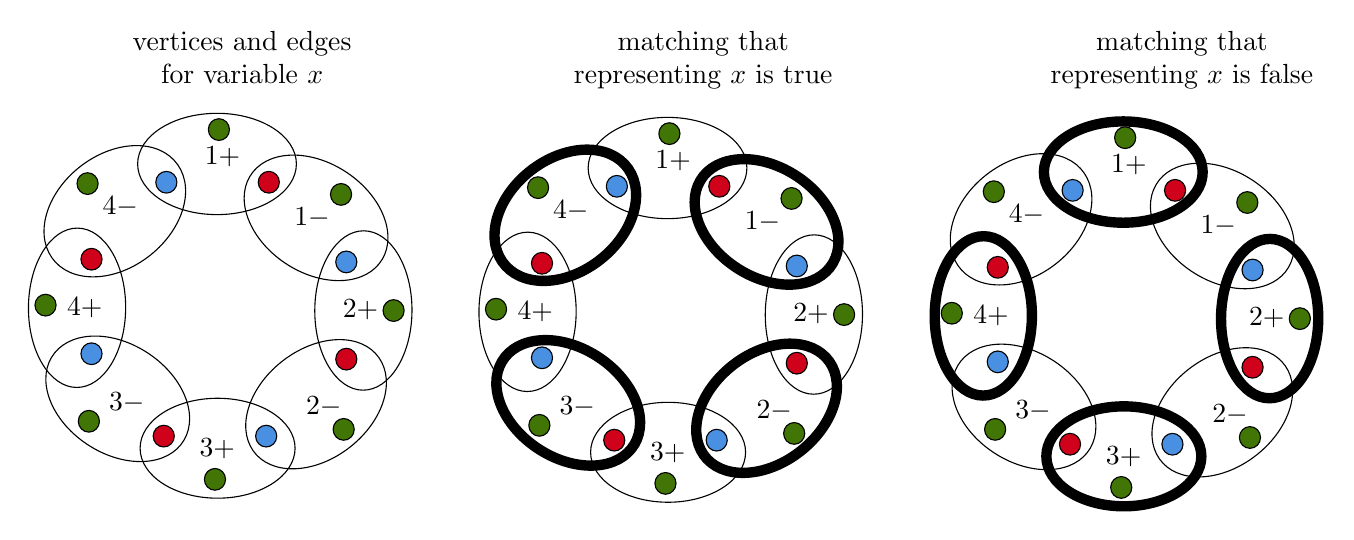
\begin{tikzpicture}[x=0.5pt,y=0.5pt,yscale=-1,xscale=1]
%uncomment if require: \path (0,429); %set diagram left start at 0, and has height of 429

%Shape: Ellipse [id:dp7769270587227844] 
\draw  [fill={rgb, 255:red, 74; green, 144; blue, 226 }  ,fill opacity=1 ] (101.91,158.81) .. controls (101.91,154.47) and (105.33,150.96) .. (109.54,150.96) .. controls (113.76,150.96) and (117.17,154.47) .. (117.17,158.81) .. controls (117.17,163.14) and (113.76,166.66) .. (109.54,166.66) .. controls (105.33,166.66) and (101.91,163.14) .. (101.91,158.81) -- cycle ;
%Shape: Ellipse [id:dp05059412992929113] 
\draw  [fill={rgb, 255:red, 208; green, 2; blue, 27 }  ,fill opacity=1 ] (175.95,158.81) .. controls (175.95,154.47) and (179.36,150.96) .. (183.58,150.96) .. controls (187.8,150.96) and (191.21,154.47) .. (191.21,158.81) .. controls (191.21,163.14) and (187.8,166.66) .. (183.58,166.66) .. controls (179.36,166.66) and (175.95,163.14) .. (175.95,158.81) -- cycle ;
%Shape: Ellipse [id:dp9392486510933934] 
\draw  [fill={rgb, 255:red, 74; green, 144; blue, 226 }  ,fill opacity=1 ] (47.8,282.75) .. controls (47.8,278.42) and (51.22,274.9) .. (55.44,274.9) .. controls (59.65,274.9) and (63.07,278.42) .. (63.07,282.75) .. controls (63.07,287.09) and (59.65,290.6) .. (55.44,290.6) .. controls (51.22,290.6) and (47.8,287.09) .. (47.8,282.75) -- cycle ;
%Shape: Ellipse [id:dp937505061939578] 
\draw  [fill={rgb, 255:red, 208; green, 2; blue, 27 }  ,fill opacity=1 ] (47.8,214.44) .. controls (47.8,210.1) and (51.22,206.59) .. (55.44,206.59) .. controls (59.65,206.59) and (63.07,210.1) .. (63.07,214.44) .. controls (63.07,218.77) and (59.65,222.28) .. (55.44,222.28) .. controls (51.22,222.28) and (47.8,218.77) .. (47.8,214.44) -- cycle ;
%Shape: Ellipse [id:dp3418898559465017] 
\draw  [fill={rgb, 255:red, 208; green, 2; blue, 27 }  ,fill opacity=1 ] (100.01,342.28) .. controls (100.01,337.95) and (103.43,334.44) .. (107.64,334.44) .. controls (111.86,334.44) and (115.28,337.95) .. (115.28,342.28) .. controls (115.28,346.62) and (111.86,350.13) .. (107.64,350.13) .. controls (103.43,350.13) and (100.01,346.62) .. (100.01,342.28) -- cycle ;
%Shape: Ellipse [id:dp0792417640170372] 
\draw  [fill={rgb, 255:red, 74; green, 144; blue, 226 }  ,fill opacity=1 ] (174.05,342.28) .. controls (174.05,337.95) and (177.47,334.44) .. (181.68,334.44) .. controls (185.9,334.44) and (189.31,337.95) .. (189.31,342.28) .. controls (189.31,346.62) and (185.9,350.13) .. (181.68,350.13) .. controls (177.47,350.13) and (174.05,346.62) .. (174.05,342.28) -- cycle ;
%Shape: Ellipse [id:dp7784181208836367] 
\draw  [fill={rgb, 255:red, 74; green, 144; blue, 226 }  ,fill opacity=1 ] (231.95,216.39) .. controls (231.95,212.05) and (235.37,208.54) .. (239.58,208.54) .. controls (243.8,208.54) and (247.22,212.05) .. (247.22,216.39) .. controls (247.22,220.72) and (243.8,224.24) .. (239.58,224.24) .. controls (235.37,224.24) and (231.95,220.72) .. (231.95,216.39) -- cycle ;
%Shape: Ellipse [id:dp5209312270506765] 
\draw  [fill={rgb, 255:red, 208; green, 2; blue, 27 }  ,fill opacity=1 ] (231.95,286.66) .. controls (231.95,282.32) and (235.37,278.81) .. (239.58,278.81) .. controls (243.8,278.81) and (247.22,282.32) .. (247.22,286.66) .. controls (247.22,290.99) and (243.8,294.5) .. (239.58,294.5) .. controls (235.37,294.5) and (231.95,290.99) .. (231.95,286.66) -- cycle ;
%Shape: Ellipse [id:dp3160597017262764] 
\draw  [fill={rgb, 255:red, 65; green, 117; blue, 5 }  ,fill opacity=1 ] (139.88,120.74) .. controls (139.88,116.41) and (143.29,112.9) .. (147.51,112.9) .. controls (151.73,112.9) and (155.14,116.41) .. (155.14,120.74) .. controls (155.14,125.08) and (151.73,128.59) .. (147.51,128.59) .. controls (143.29,128.59) and (139.88,125.08) .. (139.88,120.74) -- cycle ;
%Shape: Ellipse [id:dp5930658241432455] 
\draw  [fill={rgb, 255:red, 65; green, 117; blue, 5 }  ,fill opacity=1 ] (228.15,167.59) .. controls (228.15,163.26) and (231.57,159.74) .. (235.79,159.74) .. controls (240,159.74) and (243.42,163.26) .. (243.42,167.59) .. controls (243.42,171.92) and (240,175.44) .. (235.79,175.44) .. controls (231.57,175.44) and (228.15,171.92) .. (228.15,167.59) -- cycle ;
%Shape: Ellipse [id:dp735085873973755] 
\draw  [fill={rgb, 255:red, 65; green, 117; blue, 5 }  ,fill opacity=1 ] (266.12,251.52) .. controls (266.12,247.19) and (269.54,243.67) .. (273.75,243.67) .. controls (277.97,243.67) and (281.39,247.19) .. (281.39,251.52) .. controls (281.39,255.86) and (277.97,259.37) .. (273.75,259.37) .. controls (269.54,259.37) and (266.12,255.86) .. (266.12,251.52) -- cycle ;
%Shape: Ellipse [id:dp02630270416437519] 
\draw  [fill={rgb, 255:red, 65; green, 117; blue, 5 }  ,fill opacity=1 ] (230.05,337.4) .. controls (230.05,333.07) and (233.47,329.56) .. (237.68,329.56) .. controls (241.9,329.56) and (245.32,333.07) .. (245.32,337.4) .. controls (245.32,341.74) and (241.9,345.25) .. (237.68,345.25) .. controls (233.47,345.25) and (230.05,341.74) .. (230.05,337.4) -- cycle ;
%Shape: Ellipse [id:dp18485588309861056] 
\draw  [fill={rgb, 255:red, 65; green, 117; blue, 5 }  ,fill opacity=1 ] (137.03,373.51) .. controls (137.03,369.18) and (140.45,365.67) .. (144.66,365.67) .. controls (148.88,365.67) and (152.3,369.18) .. (152.3,373.51) .. controls (152.3,377.85) and (148.88,381.36) .. (144.66,381.36) .. controls (140.45,381.36) and (137.03,377.85) .. (137.03,373.51) -- cycle ;
%Shape: Ellipse [id:dp8374259958133121] 
\draw  [fill={rgb, 255:red, 65; green, 117; blue, 5 }  ,fill opacity=1 ] (45.9,331.55) .. controls (45.9,327.21) and (49.32,323.7) .. (53.54,323.7) .. controls (57.75,323.7) and (61.17,327.21) .. (61.17,331.55) .. controls (61.17,335.88) and (57.75,339.4) .. (53.54,339.4) .. controls (49.32,339.4) and (45.9,335.88) .. (45.9,331.55) -- cycle ;
%Shape: Ellipse [id:dp708058297360727] 
\draw  [fill={rgb, 255:red, 65; green, 117; blue, 5 }  ,fill opacity=1 ] (14.58,247.62) .. controls (14.58,243.28) and (18,239.77) .. (22.21,239.77) .. controls (26.43,239.77) and (29.85,243.28) .. (29.85,247.62) .. controls (29.85,251.95) and (26.43,255.47) .. (22.21,255.47) .. controls (18,255.47) and (14.58,251.95) .. (14.58,247.62) -- cycle ;
%Shape: Ellipse [id:dp9781528549366821] 
\draw  [fill={rgb, 255:red, 65; green, 117; blue, 5 }  ,fill opacity=1 ] (44.96,159.78) .. controls (44.96,155.45) and (48.37,151.93) .. (52.59,151.93) .. controls (56.8,151.93) and (60.22,155.45) .. (60.22,159.78) .. controls (60.22,164.12) and (56.8,167.63) .. (52.59,167.63) .. controls (48.37,167.63) and (44.96,164.12) .. (44.96,159.78) -- cycle ;
%Shape: Ellipse [id:dp6007503928324749] 
\draw   (88.78,145.59) .. controls (88.78,125.38) and (114.46,108.99) .. (146.15,108.99) .. controls (177.83,108.99) and (203.51,125.38) .. (203.51,145.59) .. controls (203.51,165.81) and (177.83,182.2) .. (146.15,182.2) .. controls (114.46,182.2) and (88.78,165.81) .. (88.78,145.59) -- cycle ;
%Shape: Ellipse [id:dp26925532128547036] 
\draw   (90.56,351.03) .. controls (90.56,331.09) and (115.63,314.92) .. (146.56,314.92) .. controls (177.49,314.92) and (202.56,331.09) .. (202.56,351.03) .. controls (202.56,370.98) and (177.49,387.14) .. (146.56,387.14) .. controls (115.63,387.14) and (90.56,370.98) .. (90.56,351.03) -- cycle ;
%Shape: Ellipse [id:dp5556772057799917] 
\draw   (252.2,193.9) .. controls (271.6,194) and (287.2,219.87) .. (287.05,251.67) .. controls (286.89,283.47) and (271.04,309.17) .. (251.64,309.07) .. controls (232.24,308.96) and (216.64,283.1) .. (216.8,251.3) .. controls (216.95,219.5) and (232.8,193.8) .. (252.2,193.9) -- cycle ;
%Shape: Ellipse [id:dp5358666436982396] 
\draw   (45.28,191.95) .. controls (64.68,192.05) and (80.28,217.92) .. (80.12,249.72) .. controls (79.97,281.52) and (64.11,307.22) .. (44.71,307.11) .. controls (25.31,307.01) and (9.71,281.15) .. (9.87,249.35) .. controls (10.02,217.55) and (25.88,191.85) .. (45.28,191.95) -- cycle ;
%Shape: Ellipse [id:dp5360815178586529] 
\draw   (169.84,154.67) .. controls (180.97,135.82) and (211.42,133.91) .. (237.86,150.41) .. controls (264.31,166.91) and (276.72,195.56) .. (265.6,214.41) .. controls (254.47,233.26) and (224.02,235.17) .. (197.57,218.67) .. controls (171.13,202.17) and (158.71,173.52) .. (169.84,154.67) -- cycle ;
%Shape: Ellipse [id:dp4912828709878506] 
\draw   (26.51,285.45) .. controls (37.64,266.6) and (68.09,264.69) .. (94.53,281.19) .. controls (120.98,297.68) and (133.39,326.34) .. (122.27,345.19) .. controls (111.14,364.04) and (80.69,365.95) .. (54.24,349.45) .. controls (27.8,332.95) and (15.38,304.3) .. (26.51,285.45) -- cycle ;
%Shape: Ellipse [id:dp711725599176981] 
\draw   (172.22,352.8) .. controls (159.72,334.89) and (169.95,305.33) .. (195.07,286.79) .. controls (220.2,268.24) and (250.71,267.73) .. (263.21,285.64) .. controls (275.72,303.56) and (265.49,333.11) .. (240.36,351.66) .. controls (215.24,370.2) and (184.73,370.71) .. (172.22,352.8) -- cycle ;
%Shape: Ellipse [id:dp04407905885833341] 
\draw   (26.79,213.33) .. controls (13.87,194.83) and (23.77,164.8) .. (48.9,146.25) .. controls (74.02,127.71) and (104.86,127.67) .. (117.78,146.17) .. controls (130.69,164.67) and (120.8,194.7) .. (95.67,213.25) .. controls (70.54,231.79) and (39.7,231.83) .. (26.79,213.33) -- cycle ;
%Shape: Ellipse [id:dp6083089858303113] 
\draw  [fill={rgb, 255:red, 74; green, 144; blue, 226 }  ,fill opacity=1 ] (427.49,161.73) .. controls (427.49,157.4) and (430.9,153.89) .. (435.12,153.89) .. controls (439.33,153.89) and (442.75,157.4) .. (442.75,161.73) .. controls (442.75,166.07) and (439.33,169.58) .. (435.12,169.58) .. controls (430.9,169.58) and (427.49,166.07) .. (427.49,161.73) -- cycle ;
%Shape: Ellipse [id:dp890348825650377] 
\draw  [fill={rgb, 255:red, 208; green, 2; blue, 27 }  ,fill opacity=1 ] (501.52,161.73) .. controls (501.52,157.4) and (504.94,153.89) .. (509.16,153.89) .. controls (513.37,153.89) and (516.79,157.4) .. (516.79,161.73) .. controls (516.79,166.07) and (513.37,169.58) .. (509.16,169.58) .. controls (504.94,169.58) and (501.52,166.07) .. (501.52,161.73) -- cycle ;
%Shape: Ellipse [id:dp40250121602370204] 
\draw  [fill={rgb, 255:red, 74; green, 144; blue, 226 }  ,fill opacity=1 ] (373.38,285.68) .. controls (373.38,281.35) and (376.8,277.83) .. (381.01,277.83) .. controls (385.23,277.83) and (388.65,281.35) .. (388.65,285.68) .. controls (388.65,290.01) and (385.23,293.53) .. (381.01,293.53) .. controls (376.8,293.53) and (373.38,290.01) .. (373.38,285.68) -- cycle ;
%Shape: Ellipse [id:dp9443549716763927] 
\draw  [fill={rgb, 255:red, 208; green, 2; blue, 27 }  ,fill opacity=1 ] (373.38,217.36) .. controls (373.38,213.03) and (376.8,209.52) .. (381.01,209.52) .. controls (385.23,209.52) and (388.65,213.03) .. (388.65,217.36) .. controls (388.65,221.7) and (385.23,225.21) .. (381.01,225.21) .. controls (376.8,225.21) and (373.38,221.7) .. (373.38,217.36) -- cycle ;
%Shape: Ellipse [id:dp5606670420326237] 
\draw  [fill={rgb, 255:red, 208; green, 2; blue, 27 }  ,fill opacity=1 ] (425.59,345.21) .. controls (425.59,340.88) and (429,337.36) .. (433.22,337.36) .. controls (437.44,337.36) and (440.85,340.88) .. (440.85,345.21) .. controls (440.85,349.55) and (437.44,353.06) .. (433.22,353.06) .. controls (429,353.06) and (425.59,349.55) .. (425.59,345.21) -- cycle ;
%Shape: Ellipse [id:dp06528712691745298] 
\draw  [fill={rgb, 255:red, 74; green, 144; blue, 226 }  ,fill opacity=1 ] (499.63,345.21) .. controls (499.63,340.88) and (503.04,337.36) .. (507.26,337.36) .. controls (511.47,337.36) and (514.89,340.88) .. (514.89,345.21) .. controls (514.89,349.55) and (511.47,353.06) .. (507.26,353.06) .. controls (503.04,353.06) and (499.63,349.55) .. (499.63,345.21) -- cycle ;
%Shape: Ellipse [id:dp47722043615834775] 
\draw  [fill={rgb, 255:red, 74; green, 144; blue, 226 }  ,fill opacity=1 ] (557.53,219.32) .. controls (557.53,214.98) and (560.94,211.47) .. (565.16,211.47) .. controls (569.38,211.47) and (572.79,214.98) .. (572.79,219.32) .. controls (572.79,223.65) and (569.38,227.16) .. (565.16,227.16) .. controls (560.94,227.16) and (557.53,223.65) .. (557.53,219.32) -- cycle ;
%Shape: Ellipse [id:dp8993129678892711] 
\draw  [fill={rgb, 255:red, 208; green, 2; blue, 27 }  ,fill opacity=1 ] (557.53,289.58) .. controls (557.53,285.25) and (560.94,281.74) .. (565.16,281.74) .. controls (569.38,281.74) and (572.79,285.25) .. (572.79,289.58) .. controls (572.79,293.92) and (569.38,297.43) .. (565.16,297.43) .. controls (560.94,297.43) and (557.53,293.92) .. (557.53,289.58) -- cycle ;
%Shape: Ellipse [id:dp5085250317320985] 
\draw  [fill={rgb, 255:red, 65; green, 117; blue, 5 }  ,fill opacity=1 ] (465.45,123.67) .. controls (465.45,119.34) and (468.87,115.82) .. (473.09,115.82) .. controls (477.3,115.82) and (480.72,119.34) .. (480.72,123.67) .. controls (480.72,128.01) and (477.3,131.52) .. (473.09,131.52) .. controls (468.87,131.52) and (465.45,128.01) .. (465.45,123.67) -- cycle ;
%Shape: Ellipse [id:dp6599100252536534] 
\draw  [fill={rgb, 255:red, 65; green, 117; blue, 5 }  ,fill opacity=1 ] (553.73,170.52) .. controls (553.73,166.18) and (557.15,162.67) .. (561.36,162.67) .. controls (565.58,162.67) and (569,166.18) .. (569,170.52) .. controls (569,174.85) and (565.58,178.37) .. (561.36,178.37) .. controls (557.15,178.37) and (553.73,174.85) .. (553.73,170.52) -- cycle ;
%Shape: Ellipse [id:dp07000413173713671] 
\draw  [fill={rgb, 255:red, 65; green, 117; blue, 5 }  ,fill opacity=1 ] (591.7,254.45) .. controls (591.7,250.11) and (595.12,246.6) .. (599.33,246.6) .. controls (603.55,246.6) and (606.97,250.11) .. (606.97,254.45) .. controls (606.97,258.78) and (603.55,262.3) .. (599.33,262.3) .. controls (595.12,262.3) and (591.7,258.78) .. (591.7,254.45) -- cycle ;
%Shape: Ellipse [id:dp43674403352024993] 
\draw  [fill={rgb, 255:red, 65; green, 117; blue, 5 }  ,fill opacity=1 ] (555.63,340.33) .. controls (555.63,336) and (559.05,332.48) .. (563.26,332.48) .. controls (567.48,332.48) and (570.9,336) .. (570.9,340.33) .. controls (570.9,344.67) and (567.48,348.18) .. (563.26,348.18) .. controls (559.05,348.18) and (555.63,344.67) .. (555.63,340.33) -- cycle ;
%Shape: Ellipse [id:dp5868783666579171] 
\draw  [fill={rgb, 255:red, 65; green, 117; blue, 5 }  ,fill opacity=1 ] (462.61,376.44) .. controls (462.61,372.11) and (466.02,368.59) .. (470.24,368.59) .. controls (474.46,368.59) and (477.87,372.11) .. (477.87,376.44) .. controls (477.87,380.78) and (474.46,384.29) .. (470.24,384.29) .. controls (466.02,384.29) and (462.61,380.78) .. (462.61,376.44) -- cycle ;
%Shape: Ellipse [id:dp9752335873907485] 
\draw  [fill={rgb, 255:red, 65; green, 117; blue, 5 }  ,fill opacity=1 ] (371.48,334.48) .. controls (371.48,330.14) and (374.9,326.63) .. (379.12,326.63) .. controls (383.33,326.63) and (386.75,330.14) .. (386.75,334.48) .. controls (386.75,338.81) and (383.33,342.33) .. (379.12,342.33) .. controls (374.9,342.33) and (371.48,338.81) .. (371.48,334.48) -- cycle ;
%Shape: Ellipse [id:dp49750164964620147] 
\draw  [fill={rgb, 255:red, 65; green, 117; blue, 5 }  ,fill opacity=1 ] (340.16,250.55) .. controls (340.16,246.21) and (343.58,242.7) .. (347.79,242.7) .. controls (352.01,242.7) and (355.43,246.21) .. (355.43,250.55) .. controls (355.43,254.88) and (352.01,258.39) .. (347.79,258.39) .. controls (343.58,258.39) and (340.16,254.88) .. (340.16,250.55) -- cycle ;
%Shape: Ellipse [id:dp7988191736334713] 
\draw  [fill={rgb, 255:red, 65; green, 117; blue, 5 }  ,fill opacity=1 ] (370.53,162.71) .. controls (370.53,158.38) and (373.95,154.86) .. (378.17,154.86) .. controls (382.38,154.86) and (385.8,158.38) .. (385.8,162.71) .. controls (385.8,167.05) and (382.38,170.56) .. (378.17,170.56) .. controls (373.95,170.56) and (370.53,167.05) .. (370.53,162.71) -- cycle ;
%Shape: Ellipse [id:dp9678529635545928] 
\draw   (414.36,148.52) .. controls (414.36,128.31) and (440.04,111.92) .. (471.72,111.92) .. controls (503.41,111.92) and (529.09,128.31) .. (529.09,148.52) .. controls (529.09,168.74) and (503.41,185.12) .. (471.72,185.12) .. controls (440.04,185.12) and (414.36,168.74) .. (414.36,148.52) -- cycle ;
%Shape: Ellipse [id:dp008905392676544777] 
\draw   (416.14,353.96) .. controls (416.14,334.01) and (441.21,317.85) .. (472.14,317.85) .. controls (503.07,317.85) and (528.14,334.01) .. (528.14,353.96) .. controls (528.14,373.9) and (503.07,390.07) .. (472.14,390.07) .. controls (441.21,390.07) and (416.14,373.9) .. (416.14,353.96) -- cycle ;
%Shape: Ellipse [id:dp07003950650832613] 
\draw   (577.78,196.83) .. controls (597.18,196.93) and (612.78,222.79) .. (612.63,254.6) .. controls (612.47,286.4) and (596.62,312.09) .. (577.22,311.99) .. controls (557.82,311.89) and (542.22,286.03) .. (542.37,254.23) .. controls (542.53,222.43) and (558.38,196.73) .. (577.78,196.83) -- cycle ;
%Shape: Ellipse [id:dp9072668168643843] 
\draw   (370.85,194.88) .. controls (390.25,194.98) and (405.85,220.84) .. (405.7,252.64) .. controls (405.54,284.45) and (389.69,310.14) .. (370.29,310.04) .. controls (350.89,309.94) and (335.29,284.08) .. (335.45,252.28) .. controls (335.6,220.48) and (351.46,194.78) .. (370.85,194.88) -- cycle ;
%Shape: Ellipse [id:dp930849794913192] 
\draw  [line width=3.75]  (495.42,157.6) .. controls (506.54,138.75) and (537,136.84) .. (563.44,153.34) .. controls (589.88,169.84) and (602.3,198.49) .. (591.18,217.34) .. controls (580.05,236.19) and (549.59,238.1) .. (523.15,221.6) .. controls (496.71,205.1) and (484.29,176.45) .. (495.42,157.6) -- cycle ;
%Shape: Ellipse [id:dp8416913785360675] 
\draw  [line width=3.75]  (352.09,288.37) .. controls (363.21,269.52) and (393.67,267.62) .. (420.11,284.12) .. controls (446.55,300.61) and (458.97,329.27) .. (447.85,348.12) .. controls (436.72,366.97) and (406.26,368.87) .. (379.82,352.38) .. controls (353.38,335.88) and (340.96,307.22) .. (352.09,288.37) -- cycle ;
%Shape: Ellipse [id:dp8838319258664904] 
\draw  [line width=3.75]  (497.8,355.73) .. controls (485.3,337.81) and (495.53,308.26) .. (520.65,289.71) .. controls (545.78,271.17) and (576.29,270.66) .. (588.79,288.57) .. controls (601.3,306.49) and (591.07,336.04) .. (565.94,354.59) .. controls (540.82,373.13) and (510.31,373.64) .. (497.8,355.73) -- cycle ;
%Shape: Ellipse [id:dp01641236704377491] 
\draw  [line width=3.75]  (352.37,216.25) .. controls (339.45,197.75) and (349.35,167.72) .. (374.48,149.18) .. controls (399.6,130.63) and (430.44,130.6) .. (443.36,149.1) .. controls (456.27,167.6) and (446.37,197.63) .. (421.25,216.17) .. controls (396.12,234.72) and (365.28,234.76) .. (352.37,216.25) -- cycle ;
%Shape: Ellipse [id:dp16744021900590833] 
\draw  [fill={rgb, 255:red, 74; green, 144; blue, 226 }  ,fill opacity=1 ] (756.86,164.66) .. controls (756.86,160.33) and (760.28,156.81) .. (764.49,156.81) .. controls (768.71,156.81) and (772.13,160.33) .. (772.13,164.66) .. controls (772.13,169) and (768.71,172.51) .. (764.49,172.51) .. controls (760.28,172.51) and (756.86,169) .. (756.86,164.66) -- cycle ;
%Shape: Ellipse [id:dp6132675768943091] 
\draw  [fill={rgb, 255:red, 208; green, 2; blue, 27 }  ,fill opacity=1 ] (830.9,164.66) .. controls (830.9,160.33) and (834.32,156.81) .. (838.53,156.81) .. controls (842.75,156.81) and (846.17,160.33) .. (846.17,164.66) .. controls (846.17,169) and (842.75,172.51) .. (838.53,172.51) .. controls (834.32,172.51) and (830.9,169) .. (830.9,164.66) -- cycle ;
%Shape: Ellipse [id:dp19298763030748733] 
\draw  [fill={rgb, 255:red, 74; green, 144; blue, 226 }  ,fill opacity=1 ] (702.76,288.61) .. controls (702.76,284.27) and (706.17,280.76) .. (710.39,280.76) .. controls (714.61,280.76) and (718.02,284.27) .. (718.02,288.61) .. controls (718.02,292.94) and (714.61,296.46) .. (710.39,296.46) .. controls (706.17,296.46) and (702.76,292.94) .. (702.76,288.61) -- cycle ;
%Shape: Ellipse [id:dp39286201432256407] 
\draw  [fill={rgb, 255:red, 208; green, 2; blue, 27 }  ,fill opacity=1 ] (702.76,220.29) .. controls (702.76,215.96) and (706.17,212.44) .. (710.39,212.44) .. controls (714.61,212.44) and (718.02,215.96) .. (718.02,220.29) .. controls (718.02,224.63) and (714.61,228.14) .. (710.39,228.14) .. controls (706.17,228.14) and (702.76,224.63) .. (702.76,220.29) -- cycle ;
%Shape: Ellipse [id:dp7495216422139424] 
\draw  [fill={rgb, 255:red, 208; green, 2; blue, 27 }  ,fill opacity=1 ] (754.96,348.14) .. controls (754.96,343.81) and (758.38,340.29) .. (762.6,340.29) .. controls (766.81,340.29) and (770.23,343.81) .. (770.23,348.14) .. controls (770.23,352.47) and (766.81,355.99) .. (762.6,355.99) .. controls (758.38,355.99) and (754.96,352.47) .. (754.96,348.14) -- cycle ;
%Shape: Ellipse [id:dp09555579449510876] 
\draw  [fill={rgb, 255:red, 74; green, 144; blue, 226 }  ,fill opacity=1 ] (829,348.14) .. controls (829,343.81) and (832.42,340.29) .. (836.63,340.29) .. controls (840.85,340.29) and (844.27,343.81) .. (844.27,348.14) .. controls (844.27,352.47) and (840.85,355.99) .. (836.63,355.99) .. controls (832.42,355.99) and (829,352.47) .. (829,348.14) -- cycle ;
%Shape: Ellipse [id:dp20067163474124583] 
\draw  [fill={rgb, 255:red, 74; green, 144; blue, 226 }  ,fill opacity=1 ] (886.9,222.24) .. controls (886.9,217.91) and (890.32,214.39) .. (894.54,214.39) .. controls (898.75,214.39) and (902.17,217.91) .. (902.17,222.24) .. controls (902.17,226.58) and (898.75,230.09) .. (894.54,230.09) .. controls (890.32,230.09) and (886.9,226.58) .. (886.9,222.24) -- cycle ;
%Shape: Ellipse [id:dp17345036369265776] 
\draw  [fill={rgb, 255:red, 208; green, 2; blue, 27 }  ,fill opacity=1 ] (886.9,292.51) .. controls (886.9,288.18) and (890.32,284.66) .. (894.54,284.66) .. controls (898.75,284.66) and (902.17,288.18) .. (902.17,292.51) .. controls (902.17,296.85) and (898.75,300.36) .. (894.54,300.36) .. controls (890.32,300.36) and (886.9,296.85) .. (886.9,292.51) -- cycle ;
%Shape: Ellipse [id:dp7073724427919807] 
\draw  [fill={rgb, 255:red, 65; green, 117; blue, 5 }  ,fill opacity=1 ] (794.83,126.6) .. controls (794.83,122.27) and (798.25,118.75) .. (802.46,118.75) .. controls (806.68,118.75) and (810.1,122.27) .. (810.1,126.6) .. controls (810.1,130.94) and (806.68,134.45) .. (802.46,134.45) .. controls (798.25,134.45) and (794.83,130.94) .. (794.83,126.6) -- cycle ;
%Shape: Ellipse [id:dp4220436783672431] 
\draw  [fill={rgb, 255:red, 65; green, 117; blue, 5 }  ,fill opacity=1 ] (883.11,173.45) .. controls (883.11,169.11) and (886.52,165.6) .. (890.74,165.6) .. controls (894.95,165.6) and (898.37,169.11) .. (898.37,173.45) .. controls (898.37,177.78) and (894.95,181.29) .. (890.74,181.29) .. controls (886.52,181.29) and (883.11,177.78) .. (883.11,173.45) -- cycle ;
%Shape: Ellipse [id:dp8290671226280728] 
\draw  [fill={rgb, 255:red, 65; green, 117; blue, 5 }  ,fill opacity=1 ] (921.07,257.38) .. controls (921.07,253.04) and (924.49,249.53) .. (928.71,249.53) .. controls (932.92,249.53) and (936.34,253.04) .. (936.34,257.38) .. controls (936.34,261.71) and (932.92,265.23) .. (928.71,265.23) .. controls (924.49,265.23) and (921.07,261.71) .. (921.07,257.38) -- cycle ;
%Shape: Ellipse [id:dp9254476651114719] 
\draw  [fill={rgb, 255:red, 65; green, 117; blue, 5 }  ,fill opacity=1 ] (885,343.26) .. controls (885,338.93) and (888.42,335.41) .. (892.64,335.41) .. controls (896.85,335.41) and (900.27,338.93) .. (900.27,343.26) .. controls (900.27,347.6) and (896.85,351.11) .. (892.64,351.11) .. controls (888.42,351.11) and (885,347.6) .. (885,343.26) -- cycle ;
%Shape: Ellipse [id:dp7464040164769312] 
\draw  [fill={rgb, 255:red, 65; green, 117; blue, 5 }  ,fill opacity=1 ] (791.98,379.37) .. controls (791.98,375.04) and (795.4,371.52) .. (799.61,371.52) .. controls (803.83,371.52) and (807.25,375.04) .. (807.25,379.37) .. controls (807.25,383.7) and (803.83,387.22) .. (799.61,387.22) .. controls (795.4,387.22) and (791.98,383.7) .. (791.98,379.37) -- cycle ;
%Shape: Ellipse [id:dp7609857898703889] 
\draw  [fill={rgb, 255:red, 65; green, 117; blue, 5 }  ,fill opacity=1 ] (700.86,337.4) .. controls (700.86,333.07) and (704.28,329.56) .. (708.49,329.56) .. controls (712.71,329.56) and (716.12,333.07) .. (716.12,337.4) .. controls (716.12,341.74) and (712.71,345.25) .. (708.49,345.25) .. controls (704.28,345.25) and (700.86,341.74) .. (700.86,337.4) -- cycle ;
%Shape: Ellipse [id:dp08987759175883347] 
\draw  [fill={rgb, 255:red, 65; green, 117; blue, 5 }  ,fill opacity=1 ] (669.53,253.47) .. controls (669.53,249.14) and (672.95,245.63) .. (677.17,245.63) .. controls (681.38,245.63) and (684.8,249.14) .. (684.8,253.47) .. controls (684.8,257.81) and (681.38,261.32) .. (677.17,261.32) .. controls (672.95,261.32) and (669.53,257.81) .. (669.53,253.47) -- cycle ;
%Shape: Ellipse [id:dp42832742571541016] 
\draw  [fill={rgb, 255:red, 65; green, 117; blue, 5 }  ,fill opacity=1 ] (699.91,165.64) .. controls (699.91,161.3) and (703.33,157.79) .. (707.54,157.79) .. controls (711.76,157.79) and (715.17,161.3) .. (715.17,165.64) .. controls (715.17,169.97) and (711.76,173.49) .. (707.54,173.49) .. controls (703.33,173.49) and (699.91,169.97) .. (699.91,165.64) -- cycle ;
%Shape: Ellipse [id:dp41724709745441757] 
\draw  [line width=3.75]  (743.73,151.45) .. controls (743.73,131.24) and (769.41,114.85) .. (801.1,114.85) .. controls (832.78,114.85) and (858.47,131.24) .. (858.47,151.45) .. controls (858.47,171.66) and (832.78,188.05) .. (801.1,188.05) .. controls (769.41,188.05) and (743.73,171.66) .. (743.73,151.45) -- cycle ;
%Shape: Ellipse [id:dp11424099773058216] 
\draw  [line width=3.75]  (745.51,356.89) .. controls (745.51,336.94) and (770.58,320.77) .. (801.51,320.77) .. controls (832.44,320.77) and (857.52,336.94) .. (857.52,356.89) .. controls (857.52,376.83) and (832.44,393) .. (801.51,393) .. controls (770.58,393) and (745.51,376.83) .. (745.51,356.89) -- cycle ;
%Shape: Ellipse [id:dp8705526186635797] 
\draw  [line width=3.75]  (907.16,199.76) .. controls (926.56,199.86) and (942.16,225.72) .. (942,257.52) .. controls (941.85,289.33) and (925.99,315.02) .. (906.59,314.92) .. controls (887.19,314.82) and (871.59,288.96) .. (871.75,257.16) .. controls (871.9,225.35) and (887.76,199.66) .. (907.16,199.76) -- cycle ;
%Shape: Ellipse [id:dp06459059617213647] 
\draw  [line width=3.75]  (700.23,197.81) .. controls (719.63,197.91) and (735.23,223.77) .. (735.07,255.57) .. controls (734.92,287.37) and (719.07,313.07) .. (699.67,312.97) .. controls (680.27,312.87) and (664.67,287.01) .. (664.82,255.2) .. controls (664.98,223.4) and (680.83,197.71) .. (700.23,197.81) -- cycle ;
%Shape: Ellipse [id:dp449321798697773] 
\draw   (824.79,160.53) .. controls (835.92,141.68) and (866.37,139.77) .. (892.82,156.27) .. controls (919.26,172.76) and (931.68,201.42) .. (920.55,220.27) .. controls (909.43,239.12) and (878.97,241.03) .. (852.53,224.53) .. controls (826.08,208.03) and (813.67,179.38) .. (824.79,160.53) -- cycle ;
%Shape: Ellipse [id:dp0950198302577433] 
\draw   (681.46,291.3) .. controls (692.59,272.45) and (723.04,270.55) .. (749.49,287.04) .. controls (775.93,303.54) and (788.35,332.2) .. (777.22,351.05) .. controls (766.09,369.9) and (735.64,371.8) .. (709.2,355.3) .. controls (682.75,338.81) and (670.34,310.15) .. (681.46,291.3) -- cycle ;
%Shape: Ellipse [id:dp9675062670883935] 
\draw   (827.18,358.66) .. controls (814.67,340.74) and (824.9,311.19) .. (850.03,292.64) .. controls (875.15,274.1) and (905.66,273.59) .. (918.17,291.5) .. controls (930.67,309.41) and (920.44,338.97) .. (895.32,357.51) .. controls (870.19,376.06) and (839.68,376.57) .. (827.18,358.66) -- cycle ;
%Shape: Ellipse [id:dp5573694020123918] 
\draw   (681.74,219.18) .. controls (668.83,200.68) and (678.72,170.65) .. (703.85,152.11) .. controls (728.98,133.56) and (759.81,133.53) .. (772.73,152.03) .. controls (785.65,170.53) and (775.75,200.56) .. (750.62,219.1) .. controls (725.5,237.65) and (694.66,237.68) .. (681.74,219.18) -- cycle ;

% Text Node
\draw (135.5,131.23) node [anchor=north west][inner sep=0.75pt]   [align=left] {$\displaystyle 1+$};
% Text Node
\draw (200.07,175.15) node [anchor=north west][inner sep=0.75pt]   [align=left] {$\displaystyle 1-$};
% Text Node
\draw (235.17,241.51) node [anchor=north west][inner sep=0.75pt]   [align=left] {$\displaystyle 2+$};
% Text Node
\draw (208.62,311.78) node [anchor=north west][inner sep=0.75pt]   [align=left] {$\displaystyle 2-$};
% Text Node
\draw (131.7,342.03) node [anchor=north west][inner sep=0.75pt]   [align=left] {$\displaystyle 3+$};
% Text Node
\draw (66.23,308.85) node [anchor=north west][inner sep=0.75pt]   [align=left] {$\displaystyle 3-$};
% Text Node
\draw (35.83,240.54) node [anchor=north west][inner sep=0.75pt]   [align=left] {$\displaystyle 4+$};
% Text Node
\draw (61.49,167.34) node [anchor=north west][inner sep=0.75pt]   [align=left] {$\displaystyle 4-$};
% Text Node
\draw (461.08,134.16) node [anchor=north west][inner sep=0.75pt]   [align=left] {$\displaystyle 1+$};
% Text Node
\draw (525.65,178.08) node [anchor=north west][inner sep=0.75pt]   [align=left] {$\displaystyle 1-$};
% Text Node
\draw (560.75,244.44) node [anchor=north west][inner sep=0.75pt]   [align=left] {$\displaystyle 2+$};
% Text Node
\draw (534.19,314.71) node [anchor=north west][inner sep=0.75pt]   [align=left] {$\displaystyle 2-$};
% Text Node
\draw (457.28,344.96) node [anchor=north west][inner sep=0.75pt]   [align=left] {$\displaystyle 3+$};
% Text Node
\draw (391.81,311.78) node [anchor=north west][inner sep=0.75pt]   [align=left] {$\displaystyle 3-$};
% Text Node
\draw (361.41,243.46) node [anchor=north west][inner sep=0.75pt]   [align=left] {$\displaystyle 4+$};
% Text Node
\draw (387.07,170.27) node [anchor=north west][inner sep=0.75pt]   [align=left] {$\displaystyle 4-$};
% Text Node
\draw (790.45,137.09) node [anchor=north west][inner sep=0.75pt]   [align=left] {$\displaystyle 1+$};
% Text Node
\draw (855.03,181) node [anchor=north west][inner sep=0.75pt]   [align=left] {$\displaystyle 1-$};
% Text Node
\draw (890.12,247.37) node [anchor=north west][inner sep=0.75pt]   [align=left] {$\displaystyle 2+$};
% Text Node
\draw (863.57,317.64) node [anchor=north west][inner sep=0.75pt]   [align=left] {$\displaystyle 2-$};
% Text Node
\draw (786.66,347.89) node [anchor=north west][inner sep=0.75pt]   [align=left] {$\displaystyle 3+$};
% Text Node
\draw (721.19,314.71) node [anchor=north west][inner sep=0.75pt]   [align=left] {$\displaystyle 3-$};
% Text Node
\draw (690.79,246.39) node [anchor=north west][inner sep=0.75pt]   [align=left] {$\displaystyle 4+$};
% Text Node
\draw (716.44,173.2) node [anchor=north west][inner sep=0.75pt]   [align=left] {$\displaystyle 4-$};
% Text Node
\draw (74,47.5) node [anchor=north west][inner sep=0.75pt]   [align=left] {\begin{minipage}[lt]{88.35pt}\setlength\topsep{0pt}
\begin{center}
vertices and edges\\for variable $\displaystyle x$
\end{center}

\end{minipage}};
% Text Node
\draw (397,47.5) node [anchor=north west][inner sep=0.75pt]   [align=left] {\begin{minipage}[lt]{98.64pt}\setlength\topsep{0pt}
\begin{center}
matching that\\representing $\displaystyle x$ is true
\end{center}

\end{minipage}};
% Text Node
\draw (739,47.5) node [anchor=north west][inner sep=0.75pt]   [align=left] {\begin{minipage}[lt]{102.61pt}\setlength\topsep{0pt}
\begin{center}
matching that\\representing $\displaystyle x$ is false
\end{center}

\end{minipage}};


\end{tikzpicture}

}
\caption{Left: the ``switch'' created for a single variable $x$, assuming the
given 3SAT instances contains 4 clauses. We color vertices
in $X$, $Y$, and $Z$ blue, red, and green respectively. The edges~(i.e., triples)
are represented as circles. Middle: the situation where $x$ is true.
Right: the situation where $x$ is false.}
\label{fig:3dvar}
\end{figure}

Next, we model clauses. For each clause $C_j$, $j=1,2,\cdots,n$, we first add one blue vertex one red vertex, forming a blue-red 
pair for $C_j$.
We then add 3 edges/triples, corresponding to the 3 literals in $C_j$.
If a literal is $x_i$, we add an edge consisting of the blue-red pair and the $j+$ green vertex in the switch for $x_i$;
if a literal is $\overline{x_i}$, we add an edge consisting of the blue-red pair and the $j-$ green vertex in the switch for $x_i$.
See Figure~\ref{fig:3dclauses}.

\begin{figure}[!h]
\centering{

\tikzset{every picture/.style={line width=0.75pt}} %set default line width to 0.75pt        

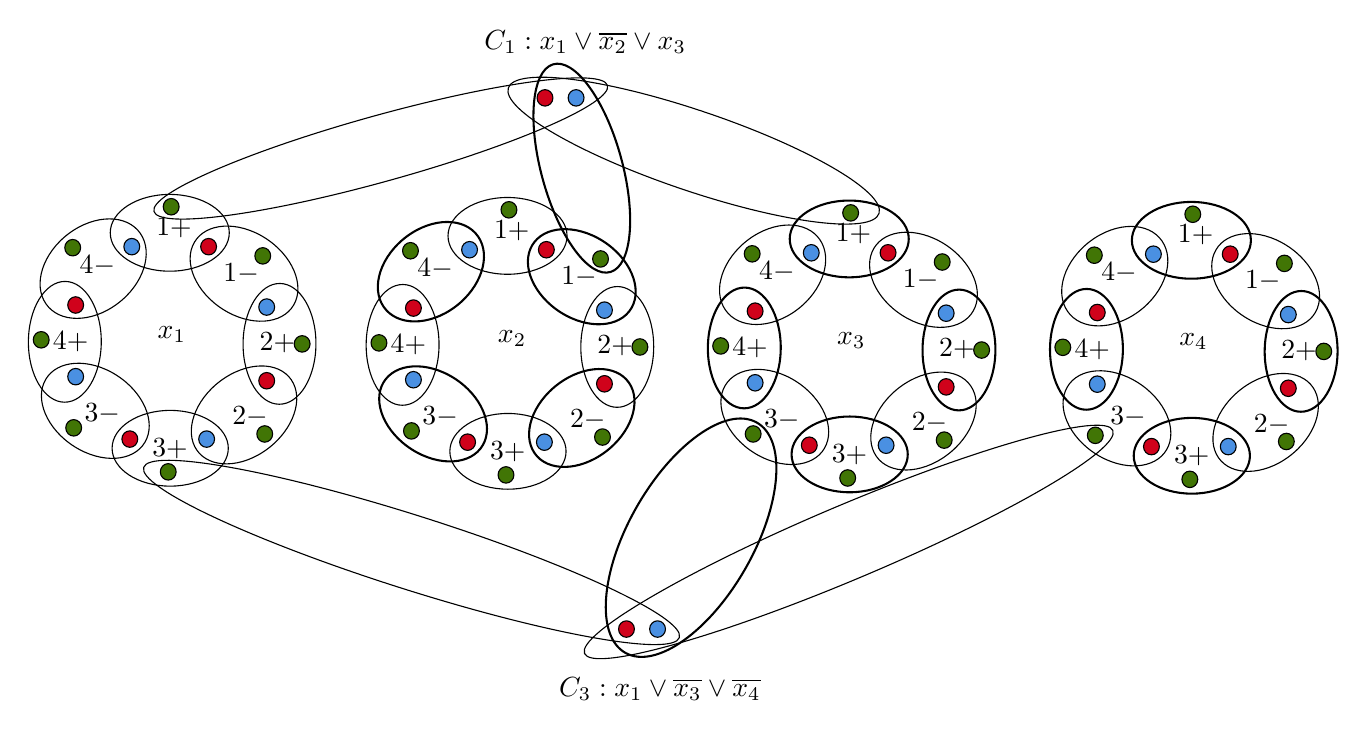
\begin{tikzpicture}[x=0.5pt,y=0.5pt,yscale=-1,xscale=1]
%uncomment if require: \path (0,586); %set diagram left start at 0, and has height of 586

%Shape: Ellipse [id:dp7769270587227844] 
\draw  [fill={rgb, 255:red, 74; green, 144; blue, 226 }  ,fill opacity=1 ] (84.87,160.76) .. controls (84.87,157.47) and (87.44,154.81) .. (90.6,154.81) .. controls (93.76,154.81) and (96.32,157.47) .. (96.32,160.76) .. controls (96.32,164.04) and (93.76,166.71) .. (90.6,166.71) .. controls (87.44,166.71) and (84.87,164.04) .. (84.87,160.76) -- cycle ;
%Shape: Ellipse [id:dp05059412992929113] 
\draw  [fill={rgb, 255:red, 208; green, 2; blue, 27 }  ,fill opacity=1 ] (140.38,160.76) .. controls (140.38,157.47) and (142.95,154.81) .. (146.11,154.81) .. controls (149.27,154.81) and (151.83,157.47) .. (151.83,160.76) .. controls (151.83,164.04) and (149.27,166.71) .. (146.11,166.71) .. controls (142.95,166.71) and (140.38,164.04) .. (140.38,160.76) -- cycle ;
%Shape: Ellipse [id:dp9392486510933934] 
\draw  [fill={rgb, 255:red, 74; green, 144; blue, 226 }  ,fill opacity=1 ] (44.31,254.7) .. controls (44.31,251.42) and (46.87,248.75) .. (50.03,248.75) .. controls (53.19,248.75) and (55.76,251.42) .. (55.76,254.7) .. controls (55.76,257.99) and (53.19,260.65) .. (50.03,260.65) .. controls (46.87,260.65) and (44.31,257.99) .. (44.31,254.7) -- cycle ;
%Shape: Ellipse [id:dp937505061939578] 
\draw  [fill={rgb, 255:red, 208; green, 2; blue, 27 }  ,fill opacity=1 ] (44.31,202.92) .. controls (44.31,199.64) and (46.87,196.97) .. (50.03,196.97) .. controls (53.19,196.97) and (55.76,199.64) .. (55.76,202.92) .. controls (55.76,206.21) and (53.19,208.87) .. (50.03,208.87) .. controls (46.87,208.87) and (44.31,206.21) .. (44.31,202.92) -- cycle ;
%Shape: Ellipse [id:dp3418898559465017] 
\draw  [fill={rgb, 255:red, 208; green, 2; blue, 27 }  ,fill opacity=1 ] (83.45,299.82) .. controls (83.45,296.54) and (86.01,293.88) .. (89.17,293.88) .. controls (92.33,293.88) and (94.9,296.54) .. (94.9,299.82) .. controls (94.9,303.11) and (92.33,305.77) .. (89.17,305.77) .. controls (86.01,305.77) and (83.45,303.11) .. (83.45,299.82) -- cycle ;
%Shape: Ellipse [id:dp0792417640170372] 
\draw  [fill={rgb, 255:red, 74; green, 144; blue, 226 }  ,fill opacity=1 ] (138.96,299.82) .. controls (138.96,296.54) and (141.52,293.88) .. (144.68,293.88) .. controls (147.84,293.88) and (150.41,296.54) .. (150.41,299.82) .. controls (150.41,303.11) and (147.84,305.77) .. (144.68,305.77) .. controls (141.52,305.77) and (138.96,303.11) .. (138.96,299.82) -- cycle ;
%Shape: Ellipse [id:dp7784181208836367] 
\draw  [fill={rgb, 255:red, 74; green, 144; blue, 226 }  ,fill opacity=1 ] (182.37,204.4) .. controls (182.37,201.12) and (184.93,198.45) .. (188.1,198.45) .. controls (191.26,198.45) and (193.82,201.12) .. (193.82,204.4) .. controls (193.82,207.69) and (191.26,210.35) .. (188.1,210.35) .. controls (184.93,210.35) and (182.37,207.69) .. (182.37,204.4) -- cycle ;
%Shape: Ellipse [id:dp5209312270506765] 
\draw  [fill={rgb, 255:red, 208; green, 2; blue, 27 }  ,fill opacity=1 ] (182.37,257.66) .. controls (182.37,254.38) and (184.93,251.71) .. (188.1,251.71) .. controls (191.26,251.71) and (193.82,254.38) .. (193.82,257.66) .. controls (193.82,260.95) and (191.26,263.61) .. (188.1,263.61) .. controls (184.93,263.61) and (182.37,260.95) .. (182.37,257.66) -- cycle ;
%Shape: Ellipse [id:dp3160597017262764] 
\draw  [fill={rgb, 255:red, 65; green, 117; blue, 5 }  ,fill opacity=1 ] (113.34,131.91) .. controls (113.34,128.62) and (115.9,125.96) .. (119.06,125.96) .. controls (122.22,125.96) and (124.79,128.62) .. (124.79,131.91) .. controls (124.79,135.2) and (122.22,137.86) .. (119.06,137.86) .. controls (115.9,137.86) and (113.34,135.2) .. (113.34,131.91) -- cycle ;
%Shape: Ellipse [id:dp5930658241432455] 
\draw  [fill={rgb, 255:red, 65; green, 117; blue, 5 }  ,fill opacity=1 ] (179.53,167.42) .. controls (179.53,164.13) and (182.09,161.47) .. (185.25,161.47) .. controls (188.41,161.47) and (190.97,164.13) .. (190.97,167.42) .. controls (190.97,170.7) and (188.41,173.36) .. (185.25,173.36) .. controls (182.09,173.36) and (179.53,170.7) .. (179.53,167.42) -- cycle ;
%Shape: Ellipse [id:dp735085873973755] 
\draw  [fill={rgb, 255:red, 65; green, 117; blue, 5 }  ,fill opacity=1 ] (207.99,231.03) .. controls (207.99,227.75) and (210.55,225.08) .. (213.72,225.08) .. controls (216.88,225.08) and (219.44,227.75) .. (219.44,231.03) .. controls (219.44,234.32) and (216.88,236.98) .. (213.72,236.98) .. controls (210.55,236.98) and (207.99,234.32) .. (207.99,231.03) -- cycle ;
%Shape: Ellipse [id:dp02630270416437519] 
\draw  [fill={rgb, 255:red, 65; green, 117; blue, 5 }  ,fill opacity=1 ] (180.95,296.13) .. controls (180.95,292.84) and (183.51,290.18) .. (186.67,290.18) .. controls (189.83,290.18) and (192.4,292.84) .. (192.4,296.13) .. controls (192.4,299.41) and (189.83,302.07) .. (186.67,302.07) .. controls (183.51,302.07) and (180.95,299.41) .. (180.95,296.13) -- cycle ;
%Shape: Ellipse [id:dp18485588309861056] 
\draw  [fill={rgb, 255:red, 65; green, 117; blue, 5 }  ,fill opacity=1 ] (111.21,323.49) .. controls (111.21,320.21) and (113.77,317.55) .. (116.93,317.55) .. controls (120.09,317.55) and (122.65,320.21) .. (122.65,323.49) .. controls (122.65,326.78) and (120.09,329.44) .. (116.93,329.44) .. controls (113.77,329.44) and (111.21,326.78) .. (111.21,323.49) -- cycle ;
%Shape: Ellipse [id:dp8374259958133121] 
\draw  [fill={rgb, 255:red, 65; green, 117; blue, 5 }  ,fill opacity=1 ] (42.89,291.69) .. controls (42.89,288.4) and (45.45,285.74) .. (48.61,285.74) .. controls (51.77,285.74) and (54.33,288.4) .. (54.33,291.69) .. controls (54.33,294.97) and (51.77,297.64) .. (48.61,297.64) .. controls (45.45,297.64) and (42.89,294.97) .. (42.89,291.69) -- cycle ;
%Shape: Ellipse [id:dp708058297360727] 
\draw  [fill={rgb, 255:red, 65; green, 117; blue, 5 }  ,fill opacity=1 ] (19.4,228.07) .. controls (19.4,224.79) and (21.96,222.12) .. (25.12,222.12) .. controls (28.29,222.12) and (30.85,224.79) .. (30.85,228.07) .. controls (30.85,231.36) and (28.29,234.02) .. (25.12,234.02) .. controls (21.96,234.02) and (19.4,231.36) .. (19.4,228.07) -- cycle ;
%Shape: Ellipse [id:dp9781528549366821] 
\draw  [fill={rgb, 255:red, 65; green, 117; blue, 5 }  ,fill opacity=1 ] (42.17,161.5) .. controls (42.17,158.21) and (44.74,155.55) .. (47.9,155.55) .. controls (51.06,155.55) and (53.62,158.21) .. (53.62,161.5) .. controls (53.62,164.78) and (51.06,167.45) .. (47.9,167.45) .. controls (44.74,167.45) and (42.17,164.78) .. (42.17,161.5) -- cycle ;
%Shape: Ellipse [id:dp6007503928324749] 
\draw   (75.03,150.74) .. controls (75.03,135.42) and (94.29,123) .. (118.04,123) .. controls (141.8,123) and (161.05,135.42) .. (161.05,150.74) .. controls (161.05,166.07) and (141.8,178.49) .. (118.04,178.49) .. controls (94.29,178.49) and (75.03,166.07) .. (75.03,150.74) -- cycle ;
%Shape: Ellipse [id:dp26925532128547036] 
\draw   (76.36,306.45) .. controls (76.36,291.34) and (95.16,279.08) .. (118.35,279.08) .. controls (141.54,279.08) and (160.34,291.34) .. (160.34,306.45) .. controls (160.34,321.57) and (141.54,333.83) .. (118.35,333.83) .. controls (95.16,333.83) and (76.36,321.57) .. (76.36,306.45) -- cycle ;
%Shape: Ellipse [id:dp5556772057799917] 
\draw   (197.56,187.36) .. controls (212.1,187.44) and (223.8,207.04) .. (223.68,231.14) .. controls (223.56,255.24) and (211.68,274.72) .. (197.13,274.64) .. controls (182.59,274.57) and (170.9,254.97) .. (171.01,230.87) .. controls (171.13,206.76) and (183.02,187.29) .. (197.56,187.36) -- cycle ;
%Shape: Ellipse [id:dp5358666436982396] 
\draw   (42.42,185.88) .. controls (56.96,185.96) and (68.66,205.56) .. (68.54,229.66) .. controls (68.42,253.76) and (56.53,273.24) .. (41.99,273.17) .. controls (27.45,273.09) and (15.75,253.49) .. (15.87,229.39) .. controls (15.99,205.28) and (27.87,185.81) .. (42.42,185.88) -- cycle ;
%Shape: Ellipse [id:dp5360815178586529] 
\draw   (135.81,157.62) .. controls (144.15,143.34) and (166.98,141.89) .. (186.81,154.4) .. controls (206.63,166.9) and (215.94,188.62) .. (207.6,202.91) .. controls (199.26,217.19) and (176.42,218.64) .. (156.6,206.13) .. controls (136.77,193.63) and (127.46,171.91) .. (135.81,157.62) -- cycle ;
%Shape: Ellipse [id:dp4912828709878506] 
\draw   (28.34,256.74) .. controls (36.69,242.46) and (59.52,241.01) .. (79.35,253.52) .. controls (99.17,266.02) and (108.48,287.74) .. (100.14,302.03) .. controls (91.8,316.31) and (68.96,317.76) .. (49.14,305.25) .. controls (29.31,292.75) and (20,271.03) .. (28.34,256.74) -- cycle ;
%Shape: Ellipse [id:dp711725599176981] 
\draw   (137.6,307.8) .. controls (128.22,294.22) and (135.89,271.82) .. (154.72,257.76) .. controls (173.56,243.7) and (196.43,243.32) .. (205.81,256.89) .. controls (215.19,270.47) and (207.52,292.87) .. (188.68,306.93) .. controls (169.84,320.99) and (146.97,321.37) .. (137.6,307.8) -- cycle ;
%Shape: Ellipse [id:dp04407905885833341] 
\draw   (28.56,202.08) .. controls (18.87,188.06) and (26.29,165.3) .. (45.13,151.24) .. controls (63.97,137.19) and (87.09,137.16) .. (96.77,151.18) .. controls (106.46,165.2) and (99.04,187.97) .. (80.2,202.02) .. controls (61.36,216.08) and (38.24,216.11) .. (28.56,202.08) -- cycle ;
%Shape: Ellipse [id:dp6083089858303113] 
\draw  [fill={rgb, 255:red, 74; green, 144; blue, 226 }  ,fill opacity=1 ] (328.98,162.98) .. controls (328.98,159.69) and (331.54,157.03) .. (334.7,157.03) .. controls (337.86,157.03) and (340.42,159.69) .. (340.42,162.98) .. controls (340.42,166.26) and (337.86,168.93) .. (334.7,168.93) .. controls (331.54,168.93) and (328.98,166.26) .. (328.98,162.98) -- cycle ;
%Shape: Ellipse [id:dp890348825650377] 
\draw  [fill={rgb, 255:red, 208; green, 2; blue, 27 }  ,fill opacity=1 ] (384.48,162.98) .. controls (384.48,159.69) and (387.05,157.03) .. (390.21,157.03) .. controls (393.37,157.03) and (395.93,159.69) .. (395.93,162.98) .. controls (395.93,166.26) and (393.37,168.93) .. (390.21,168.93) .. controls (387.05,168.93) and (384.48,166.26) .. (384.48,162.98) -- cycle ;
%Shape: Ellipse [id:dp40250121602370204] 
\draw  [fill={rgb, 255:red, 74; green, 144; blue, 226 }  ,fill opacity=1 ] (288.41,256.92) .. controls (288.41,253.64) and (290.97,250.97) .. (294.13,250.97) .. controls (297.29,250.97) and (299.86,253.64) .. (299.86,256.92) .. controls (299.86,260.21) and (297.29,262.87) .. (294.13,262.87) .. controls (290.97,262.87) and (288.41,260.21) .. (288.41,256.92) -- cycle ;
%Shape: Ellipse [id:dp9443549716763927] 
\draw  [fill={rgb, 255:red, 208; green, 2; blue, 27 }  ,fill opacity=1 ] (288.41,205.14) .. controls (288.41,201.86) and (290.97,199.19) .. (294.13,199.19) .. controls (297.29,199.19) and (299.86,201.86) .. (299.86,205.14) .. controls (299.86,208.43) and (297.29,211.09) .. (294.13,211.09) .. controls (290.97,211.09) and (288.41,208.43) .. (288.41,205.14) -- cycle ;
%Shape: Ellipse [id:dp5606670420326237] 
\draw  [fill={rgb, 255:red, 208; green, 2; blue, 27 }  ,fill opacity=1 ] (327.55,302.04) .. controls (327.55,298.76) and (330.11,296.09) .. (333.27,296.09) .. controls (336.44,296.09) and (339,298.76) .. (339,302.04) .. controls (339,305.33) and (336.44,307.99) .. (333.27,307.99) .. controls (330.11,307.99) and (327.55,305.33) .. (327.55,302.04) -- cycle ;
%Shape: Ellipse [id:dp06528712691745298] 
\draw  [fill={rgb, 255:red, 74; green, 144; blue, 226 }  ,fill opacity=1 ] (383.06,302.04) .. controls (383.06,298.76) and (385.62,296.09) .. (388.78,296.09) .. controls (391.95,296.09) and (394.51,298.76) .. (394.51,302.04) .. controls (394.51,305.33) and (391.95,307.99) .. (388.78,307.99) .. controls (385.62,307.99) and (383.06,305.33) .. (383.06,302.04) -- cycle ;
%Shape: Ellipse [id:dp47722043615834775] 
\draw  [fill={rgb, 255:red, 74; green, 144; blue, 226 }  ,fill opacity=1 ] (426.47,206.62) .. controls (426.47,203.34) and (429.04,200.67) .. (432.2,200.67) .. controls (435.36,200.67) and (437.92,203.34) .. (437.92,206.62) .. controls (437.92,209.91) and (435.36,212.57) .. (432.2,212.57) .. controls (429.04,212.57) and (426.47,209.91) .. (426.47,206.62) -- cycle ;
%Shape: Ellipse [id:dp8993129678892711] 
\draw  [fill={rgb, 255:red, 208; green, 2; blue, 27 }  ,fill opacity=1 ] (426.47,259.88) .. controls (426.47,256.59) and (429.04,253.93) .. (432.2,253.93) .. controls (435.36,253.93) and (437.92,256.59) .. (437.92,259.88) .. controls (437.92,263.17) and (435.36,265.83) .. (432.2,265.83) .. controls (429.04,265.83) and (426.47,263.17) .. (426.47,259.88) -- cycle ;
%Shape: Ellipse [id:dp5085250317320985] 
\draw  [fill={rgb, 255:red, 65; green, 117; blue, 5 }  ,fill opacity=1 ] (357.44,134.13) .. controls (357.44,130.84) and (360,128.18) .. (363.16,128.18) .. controls (366.33,128.18) and (368.89,130.84) .. (368.89,134.13) .. controls (368.89,137.41) and (366.33,140.08) .. (363.16,140.08) .. controls (360,140.08) and (357.44,137.41) .. (357.44,134.13) -- cycle ;
%Shape: Ellipse [id:dp6599100252536534] 
\draw  [fill={rgb, 255:red, 65; green, 117; blue, 5 }  ,fill opacity=1 ] (423.63,169.64) .. controls (423.63,166.35) and (426.19,163.69) .. (429.35,163.69) .. controls (432.51,163.69) and (435.07,166.35) .. (435.07,169.64) .. controls (435.07,172.92) and (432.51,175.58) .. (429.35,175.58) .. controls (426.19,175.58) and (423.63,172.92) .. (423.63,169.64) -- cycle ;
%Shape: Ellipse [id:dp07000413173713671] 
\draw  [fill={rgb, 255:red, 65; green, 117; blue, 5 }  ,fill opacity=1 ] (452.09,233.25) .. controls (452.09,229.97) and (454.66,227.3) .. (457.82,227.3) .. controls (460.98,227.3) and (463.54,229.97) .. (463.54,233.25) .. controls (463.54,236.54) and (460.98,239.2) .. (457.82,239.2) .. controls (454.66,239.2) and (452.09,236.54) .. (452.09,233.25) -- cycle ;
%Shape: Ellipse [id:dp43674403352024993] 
\draw  [fill={rgb, 255:red, 65; green, 117; blue, 5 }  ,fill opacity=1 ] (425.05,298.34) .. controls (425.05,295.06) and (427.61,292.4) .. (430.77,292.4) .. controls (433.93,292.4) and (436.5,295.06) .. (436.5,298.34) .. controls (436.5,301.63) and (433.93,304.29) .. (430.77,304.29) .. controls (427.61,304.29) and (425.05,301.63) .. (425.05,298.34) -- cycle ;
%Shape: Ellipse [id:dp5868783666579171] 
\draw  [fill={rgb, 255:red, 65; green, 117; blue, 5 }  ,fill opacity=1 ] (355.31,325.71) .. controls (355.31,322.43) and (357.87,319.77) .. (361.03,319.77) .. controls (364.19,319.77) and (366.75,322.43) .. (366.75,325.71) .. controls (366.75,329) and (364.19,331.66) .. (361.03,331.66) .. controls (357.87,331.66) and (355.31,329) .. (355.31,325.71) -- cycle ;
%Shape: Ellipse [id:dp9752335873907485] 
\draw  [fill={rgb, 255:red, 65; green, 117; blue, 5 }  ,fill opacity=1 ] (286.99,293.91) .. controls (286.99,290.62) and (289.55,287.96) .. (292.71,287.96) .. controls (295.87,287.96) and (298.43,290.62) .. (298.43,293.91) .. controls (298.43,297.19) and (295.87,299.86) .. (292.71,299.86) .. controls (289.55,299.86) and (286.99,297.19) .. (286.99,293.91) -- cycle ;
%Shape: Ellipse [id:dp49750164964620147] 
\draw  [fill={rgb, 255:red, 65; green, 117; blue, 5 }  ,fill opacity=1 ] (263.5,230.29) .. controls (263.5,227.01) and (266.06,224.34) .. (269.23,224.34) .. controls (272.39,224.34) and (274.95,227.01) .. (274.95,230.29) .. controls (274.95,233.58) and (272.39,236.24) .. (269.23,236.24) .. controls (266.06,236.24) and (263.5,233.58) .. (263.5,230.29) -- cycle ;
%Shape: Ellipse [id:dp7988191736334713] 
\draw  [fill={rgb, 255:red, 65; green, 117; blue, 5 }  ,fill opacity=1 ] (286.28,163.72) .. controls (286.28,160.43) and (288.84,157.77) .. (292,157.77) .. controls (295.16,157.77) and (297.72,160.43) .. (297.72,163.72) .. controls (297.72,167) and (295.16,169.67) .. (292,169.67) .. controls (288.84,169.67) and (286.28,167) .. (286.28,163.72) -- cycle ;
%Shape: Ellipse [id:dp9678529635545928] 
\draw   (319.13,152.96) .. controls (319.13,137.64) and (338.39,125.22) .. (362.14,125.22) .. controls (385.9,125.22) and (405.15,137.64) .. (405.15,152.96) .. controls (405.15,168.29) and (385.9,180.71) .. (362.14,180.71) .. controls (338.39,180.71) and (319.13,168.29) .. (319.13,152.96) -- cycle ;
%Shape: Ellipse [id:dp008905392676544777] 
\draw   (320.46,308.67) .. controls (320.46,293.56) and (339.26,281.3) .. (362.45,281.3) .. controls (385.64,281.3) and (404.44,293.56) .. (404.44,308.67) .. controls (404.44,323.79) and (385.64,336.04) .. (362.45,336.04) .. controls (339.26,336.04) and (320.46,323.79) .. (320.46,308.67) -- cycle ;
%Shape: Ellipse [id:dp07003950650832613] 
\draw   (441.66,189.58) .. controls (456.2,189.66) and (467.9,209.26) .. (467.78,233.36) .. controls (467.66,257.46) and (455.78,276.94) .. (441.23,276.86) .. controls (426.69,276.79) and (415,257.19) .. (415.11,233.08) .. controls (415.23,208.98) and (427.12,189.5) .. (441.66,189.58) -- cycle ;
%Shape: Ellipse [id:dp9072668168643843] 
\draw   (286.52,188.1) .. controls (301.06,188.18) and (312.76,207.78) .. (312.64,231.88) .. controls (312.52,255.98) and (300.64,275.46) .. (286.09,275.38) .. controls (271.55,275.31) and (259.85,255.71) .. (259.97,231.6) .. controls (260.09,207.5) and (271.97,188.03) .. (286.52,188.1) -- cycle ;
%Shape: Ellipse [id:dp930849794913192] 
\draw  [line width=0.75]  (379.91,159.84) .. controls (388.25,145.56) and (411.08,144.11) .. (430.91,156.61) .. controls (450.73,169.12) and (460.04,190.84) .. (451.7,205.12) .. controls (443.36,219.41) and (420.53,220.86) .. (400.7,208.35) .. controls (380.87,195.85) and (371.56,174.13) .. (379.91,159.84) -- cycle ;
%Shape: Ellipse [id:dp8416913785360675] 
\draw  [line width=0.75]  (272.44,258.96) .. controls (280.79,244.68) and (303.62,243.23) .. (323.45,255.74) .. controls (343.27,268.24) and (352.58,289.96) .. (344.24,304.25) .. controls (335.9,318.53) and (313.06,319.98) .. (293.24,307.47) .. controls (273.41,294.97) and (264.1,273.25) .. (272.44,258.96) -- cycle ;
%Shape: Ellipse [id:dp8838319258664904] 
\draw  [line width=0.75]  (381.7,310.01) .. controls (372.32,296.44) and (379.99,274.03) .. (398.83,259.98) .. controls (417.66,245.92) and (440.53,245.53) .. (449.91,259.11) .. controls (459.29,272.69) and (451.62,295.09) .. (432.78,309.15) .. controls (413.95,323.2) and (391.07,323.59) .. (381.7,310.01) -- cycle ;
%Shape: Ellipse [id:dp01641236704377491] 
\draw  [line width=0.75]  (272.66,204.3) .. controls (262.97,190.28) and (270.39,167.52) .. (289.23,153.46) .. controls (308.07,139.4) and (331.19,139.38) .. (340.87,153.4) .. controls (350.56,167.42) and (343.14,190.18) .. (324.3,204.24) .. controls (305.46,218.3) and (282.34,218.32) .. (272.66,204.3) -- cycle ;
%Shape: Ellipse [id:dp16744021900590833] 
\draw  [fill={rgb, 255:red, 74; green, 144; blue, 226 }  ,fill opacity=1 ] (575.92,165.2) .. controls (575.92,161.91) and (578.48,159.25) .. (581.65,159.25) .. controls (584.81,159.25) and (587.37,161.91) .. (587.37,165.2) .. controls (587.37,168.48) and (584.81,171.15) .. (581.65,171.15) .. controls (578.48,171.15) and (575.92,168.48) .. (575.92,165.2) -- cycle ;
%Shape: Ellipse [id:dp6132675768943091] 
\draw  [fill={rgb, 255:red, 208; green, 2; blue, 27 }  ,fill opacity=1 ] (631.43,165.2) .. controls (631.43,161.91) and (633.99,159.25) .. (637.16,159.25) .. controls (640.32,159.25) and (642.88,161.91) .. (642.88,165.2) .. controls (642.88,168.48) and (640.32,171.15) .. (637.16,171.15) .. controls (633.99,171.15) and (631.43,168.48) .. (631.43,165.2) -- cycle ;
%Shape: Ellipse [id:dp19298763030748733] 
\draw  [fill={rgb, 255:red, 74; green, 144; blue, 226 }  ,fill opacity=1 ] (535.36,259.14) .. controls (535.36,255.85) and (537.92,253.19) .. (541.08,253.19) .. controls (544.24,253.19) and (546.8,255.85) .. (546.8,259.14) .. controls (546.8,262.43) and (544.24,265.09) .. (541.08,265.09) .. controls (537.92,265.09) and (535.36,262.43) .. (535.36,259.14) -- cycle ;
%Shape: Ellipse [id:dp39286201432256407] 
\draw  [fill={rgb, 255:red, 208; green, 2; blue, 27 }  ,fill opacity=1 ] (535.36,207.36) .. controls (535.36,204.08) and (537.92,201.41) .. (541.08,201.41) .. controls (544.24,201.41) and (546.8,204.08) .. (546.8,207.36) .. controls (546.8,210.65) and (544.24,213.31) .. (541.08,213.31) .. controls (537.92,213.31) and (535.36,210.65) .. (535.36,207.36) -- cycle ;
%Shape: Ellipse [id:dp7495216422139424] 
\draw  [fill={rgb, 255:red, 208; green, 2; blue, 27 }  ,fill opacity=1 ] (574.5,304.26) .. controls (574.5,300.98) and (577.06,298.31) .. (580.22,298.31) .. controls (583.38,298.31) and (585.95,300.98) .. (585.95,304.26) .. controls (585.95,307.55) and (583.38,310.21) .. (580.22,310.21) .. controls (577.06,310.21) and (574.5,307.55) .. (574.5,304.26) -- cycle ;
%Shape: Ellipse [id:dp09555579449510876] 
\draw  [fill={rgb, 255:red, 74; green, 144; blue, 226 }  ,fill opacity=1 ] (630.01,304.26) .. controls (630.01,300.98) and (632.57,298.31) .. (635.73,298.31) .. controls (638.89,298.31) and (641.45,300.98) .. (641.45,304.26) .. controls (641.45,307.55) and (638.89,310.21) .. (635.73,310.21) .. controls (632.57,310.21) and (630.01,307.55) .. (630.01,304.26) -- cycle ;
%Shape: Ellipse [id:dp20067163474124583] 
\draw  [fill={rgb, 255:red, 74; green, 144; blue, 226 }  ,fill opacity=1 ] (673.42,208.84) .. controls (673.42,205.55) and (675.98,202.89) .. (679.14,202.89) .. controls (682.3,202.89) and (684.87,205.55) .. (684.87,208.84) .. controls (684.87,212.13) and (682.3,214.79) .. (679.14,214.79) .. controls (675.98,214.79) and (673.42,212.13) .. (673.42,208.84) -- cycle ;
%Shape: Ellipse [id:dp17345036369265776] 
\draw  [fill={rgb, 255:red, 208; green, 2; blue, 27 }  ,fill opacity=1 ] (673.42,262.1) .. controls (673.42,258.81) and (675.98,256.15) .. (679.14,256.15) .. controls (682.3,256.15) and (684.87,258.81) .. (684.87,262.1) .. controls (684.87,265.38) and (682.3,268.05) .. (679.14,268.05) .. controls (675.98,268.05) and (673.42,265.38) .. (673.42,262.1) -- cycle ;
%Shape: Ellipse [id:dp7073724427919807] 
\draw  [fill={rgb, 255:red, 65; green, 117; blue, 5 }  ,fill opacity=1 ] (604.39,136.35) .. controls (604.39,133.06) and (606.95,130.4) .. (610.11,130.4) .. controls (613.27,130.4) and (615.83,133.06) .. (615.83,136.35) .. controls (615.83,139.63) and (613.27,142.3) .. (610.11,142.3) .. controls (606.95,142.3) and (604.39,139.63) .. (604.39,136.35) -- cycle ;
%Shape: Ellipse [id:dp4220436783672431] 
\draw  [fill={rgb, 255:red, 65; green, 117; blue, 5 }  ,fill opacity=1 ] (670.57,171.85) .. controls (670.57,168.57) and (673.14,165.91) .. (676.3,165.91) .. controls (679.46,165.91) and (682.02,168.57) .. (682.02,171.85) .. controls (682.02,175.14) and (679.46,177.8) .. (676.3,177.8) .. controls (673.14,177.8) and (670.57,175.14) .. (670.57,171.85) -- cycle ;
%Shape: Ellipse [id:dp8290671226280728] 
\draw  [fill={rgb, 255:red, 65; green, 117; blue, 5 }  ,fill opacity=1 ] (699.04,235.47) .. controls (699.04,232.18) and (701.6,229.52) .. (704.76,229.52) .. controls (707.92,229.52) and (710.49,232.18) .. (710.49,235.47) .. controls (710.49,238.75) and (707.92,241.42) .. (704.76,241.42) .. controls (701.6,241.42) and (699.04,238.75) .. (699.04,235.47) -- cycle ;
%Shape: Ellipse [id:dp9254476651114719] 
\draw  [fill={rgb, 255:red, 65; green, 117; blue, 5 }  ,fill opacity=1 ] (672,300.56) .. controls (672,297.28) and (674.56,294.62) .. (677.72,294.62) .. controls (680.88,294.62) and (683.44,297.28) .. (683.44,300.56) .. controls (683.44,303.85) and (680.88,306.51) .. (677.72,306.51) .. controls (674.56,306.51) and (672,303.85) .. (672,300.56) -- cycle ;
%Shape: Ellipse [id:dp7464040164769312] 
\draw  [fill={rgb, 255:red, 65; green, 117; blue, 5 }  ,fill opacity=1 ] (602.25,327.93) .. controls (602.25,324.65) and (604.82,321.98) .. (607.98,321.98) .. controls (611.14,321.98) and (613.7,324.65) .. (613.7,327.93) .. controls (613.7,331.22) and (611.14,333.88) .. (607.98,333.88) .. controls (604.82,333.88) and (602.25,331.22) .. (602.25,327.93) -- cycle ;
%Shape: Ellipse [id:dp7609857898703889] 
\draw  [fill={rgb, 255:red, 65; green, 117; blue, 5 }  ,fill opacity=1 ] (533.93,296.13) .. controls (533.93,292.84) and (536.5,290.18) .. (539.66,290.18) .. controls (542.82,290.18) and (545.38,292.84) .. (545.38,296.13) .. controls (545.38,299.41) and (542.82,302.07) .. (539.66,302.07) .. controls (536.5,302.07) and (533.93,299.41) .. (533.93,296.13) -- cycle ;
%Shape: Ellipse [id:dp08987759175883347] 
\draw  [fill={rgb, 255:red, 65; green, 117; blue, 5 }  ,fill opacity=1 ] (510.45,232.51) .. controls (510.45,229.23) and (513.01,226.56) .. (516.17,226.56) .. controls (519.33,226.56) and (521.9,229.23) .. (521.9,232.51) .. controls (521.9,235.8) and (519.33,238.46) .. (516.17,238.46) .. controls (513.01,238.46) and (510.45,235.8) .. (510.45,232.51) -- cycle ;
%Shape: Ellipse [id:dp42832742571541016] 
\draw  [fill={rgb, 255:red, 65; green, 117; blue, 5 }  ,fill opacity=1 ] (533.22,165.94) .. controls (533.22,162.65) and (535.78,159.99) .. (538.95,159.99) .. controls (542.11,159.99) and (544.67,162.65) .. (544.67,165.94) .. controls (544.67,169.22) and (542.11,171.89) .. (538.95,171.89) .. controls (535.78,171.89) and (533.22,169.22) .. (533.22,165.94) -- cycle ;
%Shape: Ellipse [id:dp41724709745441757] 
\draw  [line width=0.75]  (566.08,155.18) .. controls (566.08,139.86) and (585.33,127.44) .. (609.09,127.44) .. controls (632.84,127.44) and (652.1,139.86) .. (652.1,155.18) .. controls (652.1,170.5) and (632.84,182.92) .. (609.09,182.92) .. controls (585.33,182.92) and (566.08,170.5) .. (566.08,155.18) -- cycle ;
%Shape: Ellipse [id:dp11424099773058216] 
\draw  [line width=0.75]  (567.41,310.89) .. controls (567.41,295.77) and (586.21,283.52) .. (609.4,283.52) .. controls (632.59,283.52) and (651.39,295.77) .. (651.39,310.89) .. controls (651.39,326.01) and (632.59,338.26) .. (609.4,338.26) .. controls (586.21,338.26) and (567.41,326.01) .. (567.41,310.89) -- cycle ;
%Shape: Ellipse [id:dp8705526186635797] 
\draw  [line width=0.75]  (688.61,191.8) .. controls (703.15,191.88) and (714.85,211.48) .. (714.73,235.58) .. controls (714.61,259.68) and (702.72,279.16) .. (688.18,279.08) .. controls (673.64,279.01) and (661.94,259.41) .. (662.06,235.3) .. controls (662.18,211.2) and (674.06,191.72) .. (688.61,191.8) -- cycle ;
%Shape: Ellipse [id:dp06459059617213647] 
\draw  [line width=0.75]  (533.47,190.32) .. controls (548.01,190.4) and (559.7,210) .. (559.59,234.1) .. controls (559.47,258.2) and (547.58,277.68) .. (533.04,277.6) .. controls (518.5,277.53) and (506.8,257.93) .. (506.92,233.82) .. controls (507.04,209.72) and (518.92,190.24) .. (533.47,190.32) -- cycle ;
%Shape: Ellipse [id:dp449321798697773] 
\draw   (626.85,162.06) .. controls (635.2,147.77) and (658.03,146.33) .. (677.86,158.83) .. controls (697.68,171.34) and (706.99,193.06) .. (698.65,207.34) .. controls (690.31,221.63) and (667.47,223.08) .. (647.65,210.57) .. controls (627.82,198.07) and (618.51,176.35) .. (626.85,162.06) -- cycle ;
%Shape: Ellipse [id:dp0950198302577433] 
\draw   (519.39,261.18) .. controls (527.73,246.9) and (550.57,245.45) .. (570.39,257.95) .. controls (590.22,270.46) and (599.53,292.18) .. (591.19,306.46) .. controls (582.85,320.75) and (560.01,322.2) .. (540.19,309.69) .. controls (520.36,297.19) and (511.05,275.47) .. (519.39,261.18) -- cycle ;
%Shape: Ellipse [id:dp9675062670883935] 
\draw   (628.64,312.23) .. controls (619.27,298.66) and (626.94,276.25) .. (645.77,262.2) .. controls (664.61,248.14) and (687.48,247.75) .. (696.86,261.33) .. controls (706.24,274.91) and (698.57,297.31) .. (679.73,311.37) .. controls (660.89,325.42) and (638.02,325.81) .. (628.64,312.23) -- cycle ;
%Shape: Ellipse [id:dp5573694020123918] 
\draw   (519.6,206.52) .. controls (509.92,192.5) and (517.34,169.74) .. (536.18,155.68) .. controls (555.01,141.62) and (578.13,141.6) .. (587.82,155.62) .. controls (597.5,169.64) and (590.08,192.4) .. (571.25,206.46) .. controls (552.41,220.52) and (529.29,220.54) .. (519.6,206.52) -- cycle ;
%Shape: Ellipse [id:dp25065784220299525] 
\draw  [fill={rgb, 255:red, 74; green, 144; blue, 226 }  ,fill opacity=1 ] (823.19,166.19) .. controls (823.19,162.9) and (825.75,160.24) .. (828.91,160.24) .. controls (832.08,160.24) and (834.64,162.9) .. (834.64,166.19) .. controls (834.64,169.47) and (832.08,172.14) .. (828.91,172.14) .. controls (825.75,172.14) and (823.19,169.47) .. (823.19,166.19) -- cycle ;
%Shape: Ellipse [id:dp7910680467055109] 
\draw  [fill={rgb, 255:red, 208; green, 2; blue, 27 }  ,fill opacity=1 ] (878.7,166.19) .. controls (878.7,162.9) and (881.26,160.24) .. (884.42,160.24) .. controls (887.58,160.24) and (890.15,162.9) .. (890.15,166.19) .. controls (890.15,169.47) and (887.58,172.14) .. (884.42,172.14) .. controls (881.26,172.14) and (878.7,169.47) .. (878.7,166.19) -- cycle ;
%Shape: Ellipse [id:dp9240827172019819] 
\draw  [fill={rgb, 255:red, 74; green, 144; blue, 226 }  ,fill opacity=1 ] (782.63,260.13) .. controls (782.63,256.85) and (785.19,254.18) .. (788.35,254.18) .. controls (791.51,254.18) and (794.07,256.85) .. (794.07,260.13) .. controls (794.07,263.42) and (791.51,266.08) .. (788.35,266.08) .. controls (785.19,266.08) and (782.63,263.42) .. (782.63,260.13) -- cycle ;
%Shape: Ellipse [id:dp14073178636069206] 
\draw  [fill={rgb, 255:red, 208; green, 2; blue, 27 }  ,fill opacity=1 ] (782.63,208.35) .. controls (782.63,205.07) and (785.19,202.4) .. (788.35,202.4) .. controls (791.51,202.4) and (794.07,205.07) .. (794.07,208.35) .. controls (794.07,211.64) and (791.51,214.3) .. (788.35,214.3) .. controls (785.19,214.3) and (782.63,211.64) .. (782.63,208.35) -- cycle ;
%Shape: Ellipse [id:dp9837510065303283] 
\draw  [fill={rgb, 255:red, 208; green, 2; blue, 27 }  ,fill opacity=1 ] (821.77,305.25) .. controls (821.77,301.97) and (824.33,299.31) .. (827.49,299.31) .. controls (830.65,299.31) and (833.21,301.97) .. (833.21,305.25) .. controls (833.21,308.54) and (830.65,311.2) .. (827.49,311.2) .. controls (824.33,311.2) and (821.77,308.54) .. (821.77,305.25) -- cycle ;
%Shape: Ellipse [id:dp02011569717246453] 
\draw  [fill={rgb, 255:red, 74; green, 144; blue, 226 }  ,fill opacity=1 ] (877.28,305.25) .. controls (877.28,301.97) and (879.84,299.31) .. (883,299.31) .. controls (886.16,299.31) and (888.72,301.97) .. (888.72,305.25) .. controls (888.72,308.54) and (886.16,311.2) .. (883,311.2) .. controls (879.84,311.2) and (877.28,308.54) .. (877.28,305.25) -- cycle ;
%Shape: Ellipse [id:dp4717556556252219] 
\draw  [fill={rgb, 255:red, 74; green, 144; blue, 226 }  ,fill opacity=1 ] (920.69,209.83) .. controls (920.69,206.55) and (923.25,203.88) .. (926.41,203.88) .. controls (929.57,203.88) and (932.14,206.55) .. (932.14,209.83) .. controls (932.14,213.12) and (929.57,215.78) .. (926.41,215.78) .. controls (923.25,215.78) and (920.69,213.12) .. (920.69,209.83) -- cycle ;
%Shape: Ellipse [id:dp8978161964566234] 
\draw  [fill={rgb, 255:red, 208; green, 2; blue, 27 }  ,fill opacity=1 ] (920.69,263.09) .. controls (920.69,259.81) and (923.25,257.14) .. (926.41,257.14) .. controls (929.57,257.14) and (932.14,259.81) .. (932.14,263.09) .. controls (932.14,266.38) and (929.57,269.04) .. (926.41,269.04) .. controls (923.25,269.04) and (920.69,266.38) .. (920.69,263.09) -- cycle ;
%Shape: Ellipse [id:dp128788648712864] 
\draw  [fill={rgb, 255:red, 65; green, 117; blue, 5 }  ,fill opacity=1 ] (851.66,137.34) .. controls (851.66,134.06) and (854.22,131.39) .. (857.38,131.39) .. controls (860.54,131.39) and (863.1,134.06) .. (863.1,137.34) .. controls (863.1,140.63) and (860.54,143.29) .. (857.38,143.29) .. controls (854.22,143.29) and (851.66,140.63) .. (851.66,137.34) -- cycle ;
%Shape: Ellipse [id:dp34811463646619845] 
\draw  [fill={rgb, 255:red, 65; green, 117; blue, 5 }  ,fill opacity=1 ] (917.84,172.85) .. controls (917.84,169.56) and (920.4,166.9) .. (923.57,166.9) .. controls (926.73,166.9) and (929.29,169.56) .. (929.29,172.85) .. controls (929.29,176.13) and (926.73,178.8) .. (923.57,178.8) .. controls (920.4,178.8) and (917.84,176.13) .. (917.84,172.85) -- cycle ;
%Shape: Ellipse [id:dp7250139311324442] 
\draw  [fill={rgb, 255:red, 65; green, 117; blue, 5 }  ,fill opacity=1 ] (946.31,236.46) .. controls (946.31,233.18) and (948.87,230.51) .. (952.03,230.51) .. controls (955.19,230.51) and (957.76,233.18) .. (957.76,236.46) .. controls (957.76,239.75) and (955.19,242.41) .. (952.03,242.41) .. controls (948.87,242.41) and (946.31,239.75) .. (946.31,236.46) -- cycle ;
%Shape: Ellipse [id:dp7566709601465638] 
\draw  [fill={rgb, 255:red, 65; green, 117; blue, 5 }  ,fill opacity=1 ] (919.27,301.56) .. controls (919.27,298.27) and (921.83,295.61) .. (924.99,295.61) .. controls (928.15,295.61) and (930.71,298.27) .. (930.71,301.56) .. controls (930.71,304.84) and (928.15,307.5) .. (924.99,307.5) .. controls (921.83,307.5) and (919.27,304.84) .. (919.27,301.56) -- cycle ;
%Shape: Ellipse [id:dp2150184115356456] 
\draw  [fill={rgb, 255:red, 65; green, 117; blue, 5 }  ,fill opacity=1 ] (849.52,328.93) .. controls (849.52,325.64) and (852.09,322.98) .. (855.25,322.98) .. controls (858.41,322.98) and (860.97,325.64) .. (860.97,328.93) .. controls (860.97,332.21) and (858.41,334.87) .. (855.25,334.87) .. controls (852.09,334.87) and (849.52,332.21) .. (849.52,328.93) -- cycle ;
%Shape: Ellipse [id:dp8633078345242816] 
\draw  [fill={rgb, 255:red, 65; green, 117; blue, 5 }  ,fill opacity=1 ] (781.2,297.12) .. controls (781.2,293.83) and (783.77,291.17) .. (786.93,291.17) .. controls (790.09,291.17) and (792.65,293.83) .. (792.65,297.12) .. controls (792.65,300.4) and (790.09,303.07) .. (786.93,303.07) .. controls (783.77,303.07) and (781.2,300.4) .. (781.2,297.12) -- cycle ;
%Shape: Ellipse [id:dp5801742525930085] 
\draw  [fill={rgb, 255:red, 65; green, 117; blue, 5 }  ,fill opacity=1 ] (757.72,233.5) .. controls (757.72,230.22) and (760.28,227.55) .. (763.44,227.55) .. controls (766.6,227.55) and (769.16,230.22) .. (769.16,233.5) .. controls (769.16,236.79) and (766.6,239.45) .. (763.44,239.45) .. controls (760.28,239.45) and (757.72,236.79) .. (757.72,233.5) -- cycle ;
%Shape: Ellipse [id:dp9602566577508291] 
\draw  [fill={rgb, 255:red, 65; green, 117; blue, 5 }  ,fill opacity=1 ] (780.49,166.93) .. controls (780.49,163.64) and (783.05,160.98) .. (786.21,160.98) .. controls (789.38,160.98) and (791.94,163.64) .. (791.94,166.93) .. controls (791.94,170.21) and (789.38,172.88) .. (786.21,172.88) .. controls (783.05,172.88) and (780.49,170.21) .. (780.49,166.93) -- cycle ;
%Shape: Ellipse [id:dp006752173534121719] 
\draw  [line width=0.75]  (813.35,156.17) .. controls (813.35,140.85) and (832.6,128.43) .. (856.36,128.43) .. controls (880.11,128.43) and (899.37,140.85) .. (899.37,156.17) .. controls (899.37,171.5) and (880.11,183.92) .. (856.36,183.92) .. controls (832.6,183.92) and (813.35,171.5) .. (813.35,156.17) -- cycle ;
%Shape: Ellipse [id:dp7393061251681466] 
\draw  [line width=0.75]  (814.68,311.88) .. controls (814.68,296.77) and (833.48,284.51) .. (856.67,284.51) .. controls (879.86,284.51) and (898.66,296.77) .. (898.66,311.88) .. controls (898.66,327) and (879.86,339.26) .. (856.67,339.26) .. controls (833.48,339.26) and (814.68,327) .. (814.68,311.88) -- cycle ;
%Shape: Ellipse [id:dp11925713470610377] 
\draw  [line width=0.75]  (935.88,192.79) .. controls (950.42,192.87) and (962.11,212.47) .. (962,236.57) .. controls (961.88,260.67) and (949.99,280.15) .. (935.45,280.07) .. controls (920.91,280) and (909.21,260.4) .. (909.33,236.3) .. controls (909.45,212.19) and (921.33,192.72) .. (935.88,192.79) -- cycle ;
%Shape: Ellipse [id:dp5960326147303756] 
\draw  [line width=0.75]  (780.73,191.31) .. controls (795.28,191.39) and (806.97,210.99) .. (806.85,235.09) .. controls (806.74,259.19) and (794.85,278.67) .. (780.31,278.6) .. controls (765.76,278.52) and (754.07,258.92) .. (754.19,234.82) .. controls (754.31,210.71) and (766.19,191.24) .. (780.73,191.31) -- cycle ;
%Shape: Ellipse [id:dp8314838462829486] 
\draw   (874.12,163.05) .. controls (882.46,148.77) and (905.3,147.32) .. (925.12,159.83) .. controls (944.95,172.33) and (954.26,194.05) .. (945.92,208.34) .. controls (937.58,222.62) and (914.74,224.07) .. (894.92,211.56) .. controls (875.09,199.06) and (865.78,177.34) .. (874.12,163.05) -- cycle ;
%Shape: Ellipse [id:dp19060398565968006] 
\draw   (766.66,262.17) .. controls (775,247.89) and (797.84,246.44) .. (817.66,258.95) .. controls (837.49,271.45) and (846.8,293.17) .. (838.46,307.46) .. controls (830.11,321.74) and (807.28,323.19) .. (787.45,310.68) .. controls (767.63,298.18) and (758.32,276.46) .. (766.66,262.17) -- cycle ;
%Shape: Ellipse [id:dp09920087681450385] 
\draw   (875.91,313.23) .. controls (866.54,299.65) and (874.2,277.25) .. (893.04,263.19) .. controls (911.88,249.13) and (934.75,248.75) .. (944.13,262.32) .. controls (953.5,275.9) and (945.84,298.3) .. (927,312.36) .. controls (908.16,326.42) and (885.29,326.8) .. (875.91,313.23) -- cycle ;
%Shape: Ellipse [id:dp04310597626336976] 
\draw   (766.87,207.51) .. controls (757.19,193.49) and (764.61,170.73) .. (783.45,156.67) .. controls (802.28,142.62) and (825.4,142.59) .. (835.09,156.61) .. controls (844.77,170.63) and (837.35,193.4) .. (818.52,207.45) .. controls (799.68,221.51) and (776.56,221.54) .. (766.87,207.51) -- cycle ;
%Shape: Ellipse [id:dp7877899541521889] 
\draw  [fill={rgb, 255:red, 208; green, 2; blue, 27 }  ,fill opacity=1 ] (383.5,53.22) .. controls (383.5,49.94) and (386.07,47.28) .. (389.23,47.28) .. controls (392.39,47.28) and (394.95,49.94) .. (394.95,53.22) .. controls (394.95,56.51) and (392.39,59.17) .. (389.23,59.17) .. controls (386.07,59.17) and (383.5,56.51) .. (383.5,53.22) -- cycle ;
%Shape: Ellipse [id:dp3842821254481381] 
\draw  [fill={rgb, 255:red, 74; green, 144; blue, 226 }  ,fill opacity=1 ] (405.96,53.22) .. controls (405.96,49.94) and (408.53,47.28) .. (411.69,47.28) .. controls (414.85,47.28) and (417.41,49.94) .. (417.41,53.22) .. controls (417.41,56.51) and (414.85,59.17) .. (411.69,59.17) .. controls (408.53,59.17) and (405.96,56.51) .. (405.96,53.22) -- cycle ;
%Shape: Ellipse [id:dp8931978517008498] 
\draw  [fill={rgb, 255:red, 208; green, 2; blue, 27 }  ,fill opacity=1 ] (442.38,437.11) .. controls (442.38,433.82) and (444.94,431.16) .. (448.1,431.16) .. controls (451.26,431.16) and (453.82,433.82) .. (453.82,437.11) .. controls (453.82,440.39) and (451.26,443.06) .. (448.1,443.06) .. controls (444.94,443.06) and (442.38,440.39) .. (442.38,437.11) -- cycle ;
%Shape: Ellipse [id:dp8541035547121285] 
\draw  [fill={rgb, 255:red, 74; green, 144; blue, 226 }  ,fill opacity=1 ] (464.84,437.11) .. controls (464.84,433.82) and (467.4,431.16) .. (470.56,431.16) .. controls (473.72,431.16) and (476.28,433.82) .. (476.28,437.11) .. controls (476.28,440.39) and (473.72,443.06) .. (470.56,443.06) .. controls (467.4,443.06) and (464.84,440.39) .. (464.84,437.11) -- cycle ;
%Shape: Ellipse [id:dp14674514369207803] 
\draw   (106.63,135.32) .. controls (103.17,122.58) and (173.73,91.88) .. (264.24,66.74) .. controls (354.75,41.61) and (430.93,31.56) .. (434.39,44.3) .. controls (437.85,57.04) and (367.28,87.75) .. (276.78,112.88) .. controls (186.27,138.01) and (110.09,148.06) .. (106.63,135.32) -- cycle ;
%Shape: Ellipse [id:dp8817495012039878] 
\draw  [line width=0.75]  (394.93,29.03) .. controls (410.4,24.21) and (432.3,53.87) .. (443.83,95.29) .. controls (455.36,136.71) and (452.17,174.19) .. (436.69,179.02) .. controls (421.21,183.84) and (399.32,154.17) .. (387.79,112.76) .. controls (376.25,71.34) and (379.45,33.86) .. (394.93,29.03) -- cycle ;
%Shape: Ellipse [id:dp917845189283666] 
\draw   (362.73,45.99) .. controls (367.77,30.8) and (431.82,38.81) .. (505.79,63.88) .. controls (579.76,88.94) and (635.64,121.58) .. (630.61,136.77) .. controls (625.57,151.96) and (561.52,143.95) .. (487.55,118.89) .. controls (413.58,93.82) and (357.7,61.18) .. (362.73,45.99) -- cycle ;
%Shape: Ellipse [id:dp6605082348171832] 
\draw   (99.17,320.27) .. controls (103.56,306.15) and (193.78,322.23) .. (300.69,356.19) .. controls (407.6,390.14) and (490.71,429.11) .. (486.33,443.23) .. controls (481.94,457.35) and (391.72,441.27) .. (284.81,407.31) .. controls (177.9,373.36) and (94.79,334.39) .. (99.17,320.27) -- cycle ;
%Shape: Ellipse [id:dp4432053522466215] 
\draw  [line width=0.75]  (542.03,287.73) .. controls (563.91,299.69) and (560.5,346.7) .. (534.41,392.74) .. controls (508.33,438.78) and (469.44,466.4) .. (447.55,454.44) .. controls (425.67,442.48) and (429.08,395.46) .. (455.17,349.42) .. controls (481.25,303.39) and (520.14,275.76) .. (542.03,287.73) -- cycle ;
%Shape: Ellipse [id:dp539567380176517] 
\draw   (417.78,454.77) .. controls (412.12,441.07) and (493,393.87) .. (598.45,349.35) .. controls (703.89,304.83) and (793.96,279.85) .. (799.62,293.56) .. controls (805.28,307.26) and (724.39,354.46) .. (618.95,398.98) .. controls (513.51,443.49) and (423.44,468.48) .. (417.78,454.77) -- cycle ;

% Text Node
\draw (106.43,137.68) node [anchor=north west][inner sep=0.75pt]   [align=left] {$\displaystyle 1+$};
% Text Node
\draw (154.97,170.97) node [anchor=north west][inner sep=0.75pt]   [align=left] {$\displaystyle 1-$};
% Text Node
\draw (181.16,221.27) node [anchor=north west][inner sep=0.75pt]   [align=left] {$\displaystyle 2+$};
% Text Node
\draw (161.37,274.53) node [anchor=north west][inner sep=0.75pt]   [align=left] {$\displaystyle 2-$};
% Text Node
\draw (103.59,297.46) node [anchor=north west][inner sep=0.75pt]   [align=left] {$\displaystyle 3+$};
% Text Node
\draw (54.63,272.31) node [anchor=north west][inner sep=0.75pt]   [align=left] {$\displaystyle 3-$};
% Text Node
\draw (31.71,220.53) node [anchor=north west][inner sep=0.75pt]   [align=left] {$\displaystyle 4+$};
% Text Node
\draw (51.07,165.05) node [anchor=north west][inner sep=0.75pt]   [align=left] {$\displaystyle 4-$};
% Text Node
\draw (350.53,139.9) node [anchor=north west][inner sep=0.75pt]   [align=left] {$\displaystyle 1+$};
% Text Node
\draw (399.07,173.18) node [anchor=north west][inner sep=0.75pt]   [align=left] {$\displaystyle 1-$};
% Text Node
\draw (425.26,223.49) node [anchor=north west][inner sep=0.75pt]   [align=left] {$\displaystyle 2+$};
% Text Node
\draw (405.48,276.74) node [anchor=north west][inner sep=0.75pt]   [align=left] {$\displaystyle 2-$};
% Text Node
\draw (347.69,299.68) node [anchor=north west][inner sep=0.75pt]   [align=left] {$\displaystyle 3+$};
% Text Node
\draw (298.73,274.53) node [anchor=north west][inner sep=0.75pt]   [align=left] {$\displaystyle 3-$};
% Text Node
\draw (275.81,222.75) node [anchor=north west][inner sep=0.75pt]   [align=left] {$\displaystyle 4+$};
% Text Node
\draw (295.17,167.27) node [anchor=north west][inner sep=0.75pt]   [align=left] {$\displaystyle 4-$};
% Text Node
\draw (597.48,142.12) node [anchor=north west][inner sep=0.75pt]   [align=left] {$\displaystyle 1+$};
% Text Node
\draw (646.02,175.4) node [anchor=north west][inner sep=0.75pt]   [align=left] {$\displaystyle 1-$};
% Text Node
\draw (672.21,225.7) node [anchor=north west][inner sep=0.75pt]   [align=left] {$\displaystyle 2+$};
% Text Node
\draw (652.42,278.96) node [anchor=north west][inner sep=0.75pt]   [align=left] {$\displaystyle 2-$};
% Text Node
\draw (594.63,301.89) node [anchor=north west][inner sep=0.75pt]   [align=left] {$\displaystyle 3+$};
% Text Node
\draw (545.67,276.74) node [anchor=north west][inner sep=0.75pt]   [align=left] {$\displaystyle 3-$};
% Text Node
\draw (522.76,224.96) node [anchor=north west][inner sep=0.75pt]   [align=left] {$\displaystyle 4+$};
% Text Node
\draw (542.11,169.49) node [anchor=north west][inner sep=0.75pt]   [align=left] {$\displaystyle 4-$};
% Text Node
\draw (107.43,216.33) node [anchor=north west][inner sep=0.75pt]   [align=left] {$\displaystyle x_{1}$};
% Text Node
\draw (353.35,219.36) node [anchor=north west][inner sep=0.75pt]   [align=left] {$\displaystyle x_{2}$};
% Text Node
\draw (598.52,220.88) node [anchor=north west][inner sep=0.75pt]   [align=left] {$\displaystyle x_{3}$};
% Text Node
\draw (343.59,2.9) node [anchor=north west][inner sep=0.75pt]   [align=left] {$\displaystyle C_{1} :x_{1} \lor \overline{x_{2}} \lor x_{3}$};
% Text Node
\draw (844.75,143.11) node [anchor=north west][inner sep=0.75pt]   [align=left] {$\displaystyle 1+$};
% Text Node
\draw (893.29,176.4) node [anchor=north west][inner sep=0.75pt]   [align=left] {$\displaystyle 1-$};
% Text Node
\draw (919.47,226.7) node [anchor=north west][inner sep=0.75pt]   [align=left] {$\displaystyle 2+$};
% Text Node
\draw (899.69,279.96) node [anchor=north west][inner sep=0.75pt]   [align=left] {$\displaystyle 2-$};
% Text Node
\draw (841.9,302.89) node [anchor=north west][inner sep=0.75pt]   [align=left] {$\displaystyle 3+$};
% Text Node
\draw (795.89,274.76) node [anchor=north west][inner sep=0.75pt]   [align=left] {$\displaystyle 3-$};
% Text Node
\draw (770.02,225.96) node [anchor=north west][inner sep=0.75pt]   [align=left] {$\displaystyle 4+$};
% Text Node
\draw (789.38,170.48) node [anchor=north west][inner sep=0.75pt]   [align=left] {$\displaystyle 4-$};
% Text Node
\draw (845.78,221.87) node [anchor=north west][inner sep=0.75pt]   [align=left] {$\displaystyle x_{4}$};
% Text Node
\draw (397.54,470.1) node [anchor=north west][inner sep=0.75pt]   [align=left] {$\displaystyle C_{3} :x_{1} \lor \overline{x_{3}} \lor \overline{x_{4}}$};


\end{tikzpicture}

}
\caption{Adding vertices and edges for clauses.
The given 3SAT instance contains $n=4$ clauses, only $C_1$ and $C_3$ are illustrated~(otherwise the figure will be too messy).}
\label{fig:3dclauses}
\end{figure}

Consider a literal~($x_i$ or $\overline{x_i}$) in $C_j$ and the corresponding
edge that consists of the blue-red pair for $C_j$ and a green vertex~(either $j+$ or $j-$) in the switch for $x_i$.
Picking this edge in the matching implies that the green vertex must be freed. The freed green vertex indicates
the assignment for $x_i$, and one can verify, in either case the literal must be true, i.e., $C_j$ is satisfied.
Hence, a perfect matching that cover all vertices, particularly the blue-red pairs for clauses, gives an assignment
that satisfies all clauses. This is the intuition behind. We include a formal proof at the end.

%If a perfect matching $M$ exists, then one (and only one) of these 3 edges will be picked. %since $b$ and $r$ need to be covered. 
%Consider the literal corresponding to the picked edge must be tru
%Without loss of generality, assume that edge correspond to literal is $\overline{x_i}$.
%Consider the switch for $x_i$, where $j-$ is covered by the said edge.
%The switch for $x_i$ therefore must be picking the possibility of freeing all ``$-$'' vertices, that is, $x_i$ is false.
%Consequently, clause $C_j$ will be satisfied.
%Note also that, two clauses $C_j$ and $C_k$ cannot be satisfied by literals $x_i$ and $\overline{x_i}$~(which they should not be).
%This is because, in such case, in the switch for $x_i$, vertices $j+$ and $k-$ must be freed, which is not possible.


The last step of the algorithm is to add ``clean-up'' vertices and edges, to create an instance of perfect 3D matching where the number
of blue, red, and green vertices must be equal. So far, we have added $mn+n$ blue vertices, $mn+n$ red vertices,
and $2mn$ green vertices. We therefor add $2mn-mn-n=mn-n$ blue vertices and $mn-n$ red vertices, forming $mn-n$ blue-red clean-up pairs.
We add $(mn-n)\cdot 2mn$ new edges, by creating an edge for every clean-up blue-red pair and every green vertex.
In a perfect 3D matching of all vertices, there will be exactly $mn$ green vertices covered by edges within switches,
exactly $n$ green vertices covered by edges for clauses.
No matter what they are, we can always pick $mn-n$ clean-up edges, that is a matching, to cover the remaining $mn-n$ green vertices
and all clean-up $mn-n$ clean-up pairs.

We prove that the 3SAT instance is satisfiable if and only if the resulting perfect 3D matching instance has a perfect matching.
Assume that 3SAT is satisfiable. We decide the status of each switch
following the truth assignment. Specifically, if $x_i$ is true 
we pick edges in its switch that cover ``$-$'' green vertices, which free all ``$+$'' vertices;
if $x_i$ is false
we pick edges in its switch that cover ``$+$'' green vertices, which free all ``$-$'' vertices.
%we free all ``$+$'' green vertices by picking all edges covering ``$-$'' green vertices,
%and otherwise we free all ``$-$'' green vertices by picking edges including ``$+$'' green vertices. 
Now consider each clause $C_j$. There must be a literal that is true.
If it is in the form of $x_i$, then $x_i$ is true and hence all ``$+$'' green vertices, 
particularly $j+$, in the switch for $x_i$ must be freed.
So, we pick the edge consisting of the blue-red clause pair for $C_j$ and $j+$.
If it is in the form of $\overline{x_i}$, then $x_i$ is false and hence all ``$-$'' green vertices, 
particularly $j-$ must be freed.
So, we pick the edge that consisting of the blue-red clause pair for $C_j$ and $j-$.
Picking edges for all clauses covers all clause pairs.
The remaining green vertices and clean-up pairs can be matched as discussed above.
All picked edges form a perfect matching.

On the other side, assume that there exists a perfect matching.
We assign values to variables depending on
which edges in each switch are picked. %For each switch, depending on which vertices are freed~(there are only two cases),
We assign $x_i$ to be true, if all ``$+$'' green in its switch are freed, 
and to be false if all ``$-$'' green vertices in its switch are freed.
We now show that this truth assignment satisfied all clauses.
Consider clause $C_j$. Its blue-red clause pair must be covered by a picked edge in the matching, which corresponds to a literal in $C_j$.
The picked edge must include a freed green vertex. According to how the edges are built, 
if in $C_j$ the corresponding literal is in the form of $x_i$, then $j+$ vertex in the switch for $x_i$ is included.
Since $j+$ is freed, we know that we have assigned $x_i$ to be true, and this satisfies $C_j$.
If in $C_j$ the corresponding literal is in the form of $\overline{x_i}$, then $j-$ vertex in the switch for $x_i$ is included in the edge.
Since $j-$ is freed, we know that we have assigned $x_i$ to be false, and again this satisfies $C_j$.
